\documentclass[11pt]{article}

% Shared notes settings for Applied Machine Learning lectures (UPES).
% Keep this file free of \documentclass to allow reuse via \input.

\usepackage[utf8]{inputenc}
\usepackage[T1]{fontenc}
\usepackage{lmodern}          % scalable T1 fonts; without this pdflatex falls back
\input{glyphtounicode}        % to bitmapped EC Type 3 and the PDFs are neither
\pdfgentounicode=1            % searchable nor screen-reader friendly
\usepackage[a4paper,margin=1in]{geometry}
\usepackage{hyperref}
\usepackage{xurl}
\usepackage{booktabs}
\usepackage{amsmath}
\usepackage{amssymb}
\usepackage{listings}
\usepackage{xcolor}
\usepackage{enumitem}
\usepackage{parskip}

% Code listings (Python-oriented for this subject).
\lstset{
  language=Python,
  basicstyle=\ttfamily\small,
  keywordstyle=\color{blue},
  commentstyle=\color{gray},
  stringstyle=\color{teal},
  showstringspaces=false,
  columns=fullflexible,
  frame=single,
  framerule=0.2pt,
  breaklines=true
}

\setlist[itemize]{topsep=0.3em,itemsep=0.2em}
\setlist[enumerate]{topsep=0.3em,itemsep=0.2em}

% Simple per-section source line.
\newcommand{\notesources}[1]{\par\noindent{\small\color{gray}\textit{Sources:} \sloppy #1\par}}

% Unit-wise source strings for this subject (used by slides + notes).
% Path is relative to the lecture `latex/` folder (the compilation CWD).
\IfFileExists{../../../_shared/aml-sources.tex}{%
  % Source strings for Applied Machine Learning (CSAI2017P) — used by slides + notes.
% Prescribed texts and reference books are taken from the course syllabus.
% Support texts are the author-hosted open-access editions:
%   statlearning.com            (ISL with Python)
%   probml.github.io/pml-book   (Murphy, Probabilistic Machine Learning)
%   d2l.ai                      (Dive into Deep Learning)
%   mml-book.github.io          (Mathematics for Machine Learning)

\newcommand{\AMLRepoURL}{https://github.com/tali7c/Applied-Machine-Learning}

% --- prescribed -------------------------------------------------------------
\newcommand{\AMLPrescribed}{%
M\"uller and Guido, \textit{Introduction to Machine Learning with Python}, O'Reilly, 2016.;%
Bishop, \textit{Pattern Recognition and Machine Learning}, Springer, 2006.;%
Murphy, \textit{Machine Learning: A Probabilistic Perspective}, MIT Press, 2012.;%
Han, Kamber and Pei, \textit{Data Mining: Concepts and Techniques} (3e), Morgan Kaufmann, 2012.%
}

% --- unit-wise ---------------------------------------------------------------
\newcommand{\AMLUnitISources}{%
M\"uller and Guido, \textit{Introduction to Machine Learning with Python}, Ch. 1.;%
Bishop, \textit{Pattern Recognition and Machine Learning}, Ch. 1.;%
Murphy, \textit{Probabilistic Machine Learning: An Introduction}, MIT Press, 2022, Ch. 1.;%
Mitchell, \textit{Machine Learning}, McGraw Hill, 1997, Ch. 1.;%
Scikit-learn documentation, accessed 2026-08-04.%
}

\newcommand{\AMLUnitIISources}{%
Bishop, \textit{Pattern Recognition and Machine Learning}, \S1.5, \S4.3, \S7.1.;%
Zhang, Lipton, Li and Smola, \textit{Dive into Deep Learning}, \S3.4.;%
Shalev-Shwartz and Ben-David, \textit{Understanding Machine Learning}, Ch. 15.;%
Murphy, \textit{Probabilistic Machine Learning: An Introduction}, Ch. 5.%
}

\newcommand{\AMLUnitIIISources}{%
Zhang, Lipton, Li and Smola, \textit{Dive into Deep Learning}, Ch. 12 (Optimization Algorithms).;%
Deisenroth, Faisal and Ong, \textit{Mathematics for Machine Learning}, Ch. 7.;%
Kingma and Ba, ``Adam: A Method for Stochastic Optimization,'' ICLR 2015.;%
Ruder, ``An overview of gradient descent optimization algorithms,'' arXiv:1609.04747, 2016.%
}

\newcommand{\AMLUnitIVSources}{%
Han, Kamber and Pei, \textit{Data Mining: Concepts and Techniques} (3e), Ch. 3.;%
M\"uller and Guido, \textit{Introduction to Machine Learning with Python}, Ch. 3--4.;%
James, Witten, Hastie, Tibshirani and Taylor, \textit{An Introduction to Statistical Learning with Python}, Ch. 5--6, 12.;%
Scikit-learn documentation (preprocessing, model selection), accessed 2026-08-04.%
}

\newcommand{\AMLUnitVSources}{%
James et al., \textit{An Introduction to Statistical Learning with Python}, Ch. 3--6.;%
Bishop, \textit{Pattern Recognition and Machine Learning}, Ch. 3.;%
Deisenroth, Faisal and Ong, \textit{Mathematics for Machine Learning}, Ch. 9.;%
M\"uller and Guido, \textit{Introduction to Machine Learning with Python}, \S2.3.%
}

\newcommand{\AMLUnitVISources}{%
Han, Kamber and Pei, \textit{Data Mining: Concepts and Techniques} (3e), Ch. 8--9.;%
James et al., \textit{An Introduction to Statistical Learning with Python}, Ch. 8--9.;%
Bishop, \textit{Pattern Recognition and Machine Learning}, Ch. 4--5, 7, 14.;%
Zhang et al., \textit{Dive into Deep Learning}, Ch. 5.%
}

\newcommand{\AMLUnitVIISources}{%
Han, Kamber and Pei, \textit{Data Mining: Concepts and Techniques} (3e), Ch. 10.;%
James et al., \textit{An Introduction to Statistical Learning with Python}, Ch. 12.;%
M\"uller and Guido, \textit{Introduction to Machine Learning with Python}, \S3.5.;%
Ester, Kriegel, Sander and Xu, ``A density-based algorithm for discovering clusters (DBSCAN),'' KDD 1996.%
}

\newcommand{\AMLLabSources}{%
M\"uller and Guido, \textit{Introduction to Machine Learning with Python}, companion notebooks.;%
McKinney, \textit{Python for Data Analysis} (3e), O'Reilly, 2022.;%
Scikit-learn user guide, accessed 2026-08-04.;%
Matplotlib and Seaborn documentation, accessed 2026-08-04.%
}
%
}{%
  % Faculty copies live under `private/` so their compile CWD is different.
  \IfFileExists{../../../../public/_shared/aml-sources.tex}{%
    % Source strings for Applied Machine Learning (CSAI2017P) — used by slides + notes.
% Prescribed texts and reference books are taken from the course syllabus.
% Support texts are the author-hosted open-access editions:
%   statlearning.com            (ISL with Python)
%   probml.github.io/pml-book   (Murphy, Probabilistic Machine Learning)
%   d2l.ai                      (Dive into Deep Learning)
%   mml-book.github.io          (Mathematics for Machine Learning)

\newcommand{\AMLRepoURL}{https://github.com/tali7c/Applied-Machine-Learning}

% --- prescribed -------------------------------------------------------------
\newcommand{\AMLPrescribed}{%
M\"uller and Guido, \textit{Introduction to Machine Learning with Python}, O'Reilly, 2016.;%
Bishop, \textit{Pattern Recognition and Machine Learning}, Springer, 2006.;%
Murphy, \textit{Machine Learning: A Probabilistic Perspective}, MIT Press, 2012.;%
Han, Kamber and Pei, \textit{Data Mining: Concepts and Techniques} (3e), Morgan Kaufmann, 2012.%
}

% --- unit-wise ---------------------------------------------------------------
\newcommand{\AMLUnitISources}{%
M\"uller and Guido, \textit{Introduction to Machine Learning with Python}, Ch. 1.;%
Bishop, \textit{Pattern Recognition and Machine Learning}, Ch. 1.;%
Murphy, \textit{Probabilistic Machine Learning: An Introduction}, MIT Press, 2022, Ch. 1.;%
Mitchell, \textit{Machine Learning}, McGraw Hill, 1997, Ch. 1.;%
Scikit-learn documentation, accessed 2026-08-04.%
}

\newcommand{\AMLUnitIISources}{%
Bishop, \textit{Pattern Recognition and Machine Learning}, \S1.5, \S4.3, \S7.1.;%
Zhang, Lipton, Li and Smola, \textit{Dive into Deep Learning}, \S3.4.;%
Shalev-Shwartz and Ben-David, \textit{Understanding Machine Learning}, Ch. 15.;%
Murphy, \textit{Probabilistic Machine Learning: An Introduction}, Ch. 5.%
}

\newcommand{\AMLUnitIIISources}{%
Zhang, Lipton, Li and Smola, \textit{Dive into Deep Learning}, Ch. 12 (Optimization Algorithms).;%
Deisenroth, Faisal and Ong, \textit{Mathematics for Machine Learning}, Ch. 7.;%
Kingma and Ba, ``Adam: A Method for Stochastic Optimization,'' ICLR 2015.;%
Ruder, ``An overview of gradient descent optimization algorithms,'' arXiv:1609.04747, 2016.%
}

\newcommand{\AMLUnitIVSources}{%
Han, Kamber and Pei, \textit{Data Mining: Concepts and Techniques} (3e), Ch. 3.;%
M\"uller and Guido, \textit{Introduction to Machine Learning with Python}, Ch. 3--4.;%
James, Witten, Hastie, Tibshirani and Taylor, \textit{An Introduction to Statistical Learning with Python}, Ch. 5--6, 12.;%
Scikit-learn documentation (preprocessing, model selection), accessed 2026-08-04.%
}

\newcommand{\AMLUnitVSources}{%
James et al., \textit{An Introduction to Statistical Learning with Python}, Ch. 3--6.;%
Bishop, \textit{Pattern Recognition and Machine Learning}, Ch. 3.;%
Deisenroth, Faisal and Ong, \textit{Mathematics for Machine Learning}, Ch. 9.;%
M\"uller and Guido, \textit{Introduction to Machine Learning with Python}, \S2.3.%
}

\newcommand{\AMLUnitVISources}{%
Han, Kamber and Pei, \textit{Data Mining: Concepts and Techniques} (3e), Ch. 8--9.;%
James et al., \textit{An Introduction to Statistical Learning with Python}, Ch. 8--9.;%
Bishop, \textit{Pattern Recognition and Machine Learning}, Ch. 4--5, 7, 14.;%
Zhang et al., \textit{Dive into Deep Learning}, Ch. 5.%
}

\newcommand{\AMLUnitVIISources}{%
Han, Kamber and Pei, \textit{Data Mining: Concepts and Techniques} (3e), Ch. 10.;%
James et al., \textit{An Introduction to Statistical Learning with Python}, Ch. 12.;%
M\"uller and Guido, \textit{Introduction to Machine Learning with Python}, \S3.5.;%
Ester, Kriegel, Sander and Xu, ``A density-based algorithm for discovering clusters (DBSCAN),'' KDD 1996.%
}

\newcommand{\AMLLabSources}{%
M\"uller and Guido, \textit{Introduction to Machine Learning with Python}, companion notebooks.;%
McKinney, \textit{Python for Data Analysis} (3e), O'Reilly, 2022.;%
Scikit-learn user guide, accessed 2026-08-04.;%
Matplotlib and Seaborn documentation, accessed 2026-08-04.%
}
%
  }{%
    % Question papers live at `private/<family>/<instrument>/`.
    \IfFileExists{../../../public/_shared/aml-sources.tex}{%
      % Source strings for Applied Machine Learning (CSAI2017P) — used by slides + notes.
% Prescribed texts and reference books are taken from the course syllabus.
% Support texts are the author-hosted open-access editions:
%   statlearning.com            (ISL with Python)
%   probml.github.io/pml-book   (Murphy, Probabilistic Machine Learning)
%   d2l.ai                      (Dive into Deep Learning)
%   mml-book.github.io          (Mathematics for Machine Learning)

\newcommand{\AMLRepoURL}{https://github.com/tali7c/Applied-Machine-Learning}

% --- prescribed -------------------------------------------------------------
\newcommand{\AMLPrescribed}{%
M\"uller and Guido, \textit{Introduction to Machine Learning with Python}, O'Reilly, 2016.;%
Bishop, \textit{Pattern Recognition and Machine Learning}, Springer, 2006.;%
Murphy, \textit{Machine Learning: A Probabilistic Perspective}, MIT Press, 2012.;%
Han, Kamber and Pei, \textit{Data Mining: Concepts and Techniques} (3e), Morgan Kaufmann, 2012.%
}

% --- unit-wise ---------------------------------------------------------------
\newcommand{\AMLUnitISources}{%
M\"uller and Guido, \textit{Introduction to Machine Learning with Python}, Ch. 1.;%
Bishop, \textit{Pattern Recognition and Machine Learning}, Ch. 1.;%
Murphy, \textit{Probabilistic Machine Learning: An Introduction}, MIT Press, 2022, Ch. 1.;%
Mitchell, \textit{Machine Learning}, McGraw Hill, 1997, Ch. 1.;%
Scikit-learn documentation, accessed 2026-08-04.%
}

\newcommand{\AMLUnitIISources}{%
Bishop, \textit{Pattern Recognition and Machine Learning}, \S1.5, \S4.3, \S7.1.;%
Zhang, Lipton, Li and Smola, \textit{Dive into Deep Learning}, \S3.4.;%
Shalev-Shwartz and Ben-David, \textit{Understanding Machine Learning}, Ch. 15.;%
Murphy, \textit{Probabilistic Machine Learning: An Introduction}, Ch. 5.%
}

\newcommand{\AMLUnitIIISources}{%
Zhang, Lipton, Li and Smola, \textit{Dive into Deep Learning}, Ch. 12 (Optimization Algorithms).;%
Deisenroth, Faisal and Ong, \textit{Mathematics for Machine Learning}, Ch. 7.;%
Kingma and Ba, ``Adam: A Method for Stochastic Optimization,'' ICLR 2015.;%
Ruder, ``An overview of gradient descent optimization algorithms,'' arXiv:1609.04747, 2016.%
}

\newcommand{\AMLUnitIVSources}{%
Han, Kamber and Pei, \textit{Data Mining: Concepts and Techniques} (3e), Ch. 3.;%
M\"uller and Guido, \textit{Introduction to Machine Learning with Python}, Ch. 3--4.;%
James, Witten, Hastie, Tibshirani and Taylor, \textit{An Introduction to Statistical Learning with Python}, Ch. 5--6, 12.;%
Scikit-learn documentation (preprocessing, model selection), accessed 2026-08-04.%
}

\newcommand{\AMLUnitVSources}{%
James et al., \textit{An Introduction to Statistical Learning with Python}, Ch. 3--6.;%
Bishop, \textit{Pattern Recognition and Machine Learning}, Ch. 3.;%
Deisenroth, Faisal and Ong, \textit{Mathematics for Machine Learning}, Ch. 9.;%
M\"uller and Guido, \textit{Introduction to Machine Learning with Python}, \S2.3.%
}

\newcommand{\AMLUnitVISources}{%
Han, Kamber and Pei, \textit{Data Mining: Concepts and Techniques} (3e), Ch. 8--9.;%
James et al., \textit{An Introduction to Statistical Learning with Python}, Ch. 8--9.;%
Bishop, \textit{Pattern Recognition and Machine Learning}, Ch. 4--5, 7, 14.;%
Zhang et al., \textit{Dive into Deep Learning}, Ch. 5.%
}

\newcommand{\AMLUnitVIISources}{%
Han, Kamber and Pei, \textit{Data Mining: Concepts and Techniques} (3e), Ch. 10.;%
James et al., \textit{An Introduction to Statistical Learning with Python}, Ch. 12.;%
M\"uller and Guido, \textit{Introduction to Machine Learning with Python}, \S3.5.;%
Ester, Kriegel, Sander and Xu, ``A density-based algorithm for discovering clusters (DBSCAN),'' KDD 1996.%
}

\newcommand{\AMLLabSources}{%
M\"uller and Guido, \textit{Introduction to Machine Learning with Python}, companion notebooks.;%
McKinney, \textit{Python for Data Analysis} (3e), O'Reilly, 2022.;%
Scikit-learn user guide, accessed 2026-08-04.;%
Matplotlib and Seaborn documentation, accessed 2026-08-04.%
}
%
    }{%
      % Marking schemes live at `private/solutions/<family>/<id>/latex/`.
      \IfFileExists{../../../../../public/_shared/aml-sources.tex}{%
        % Source strings for Applied Machine Learning (CSAI2017P) — used by slides + notes.
% Prescribed texts and reference books are taken from the course syllabus.
% Support texts are the author-hosted open-access editions:
%   statlearning.com            (ISL with Python)
%   probml.github.io/pml-book   (Murphy, Probabilistic Machine Learning)
%   d2l.ai                      (Dive into Deep Learning)
%   mml-book.github.io          (Mathematics for Machine Learning)

\newcommand{\AMLRepoURL}{https://github.com/tali7c/Applied-Machine-Learning}

% --- prescribed -------------------------------------------------------------
\newcommand{\AMLPrescribed}{%
M\"uller and Guido, \textit{Introduction to Machine Learning with Python}, O'Reilly, 2016.;%
Bishop, \textit{Pattern Recognition and Machine Learning}, Springer, 2006.;%
Murphy, \textit{Machine Learning: A Probabilistic Perspective}, MIT Press, 2012.;%
Han, Kamber and Pei, \textit{Data Mining: Concepts and Techniques} (3e), Morgan Kaufmann, 2012.%
}

% --- unit-wise ---------------------------------------------------------------
\newcommand{\AMLUnitISources}{%
M\"uller and Guido, \textit{Introduction to Machine Learning with Python}, Ch. 1.;%
Bishop, \textit{Pattern Recognition and Machine Learning}, Ch. 1.;%
Murphy, \textit{Probabilistic Machine Learning: An Introduction}, MIT Press, 2022, Ch. 1.;%
Mitchell, \textit{Machine Learning}, McGraw Hill, 1997, Ch. 1.;%
Scikit-learn documentation, accessed 2026-08-04.%
}

\newcommand{\AMLUnitIISources}{%
Bishop, \textit{Pattern Recognition and Machine Learning}, \S1.5, \S4.3, \S7.1.;%
Zhang, Lipton, Li and Smola, \textit{Dive into Deep Learning}, \S3.4.;%
Shalev-Shwartz and Ben-David, \textit{Understanding Machine Learning}, Ch. 15.;%
Murphy, \textit{Probabilistic Machine Learning: An Introduction}, Ch. 5.%
}

\newcommand{\AMLUnitIIISources}{%
Zhang, Lipton, Li and Smola, \textit{Dive into Deep Learning}, Ch. 12 (Optimization Algorithms).;%
Deisenroth, Faisal and Ong, \textit{Mathematics for Machine Learning}, Ch. 7.;%
Kingma and Ba, ``Adam: A Method for Stochastic Optimization,'' ICLR 2015.;%
Ruder, ``An overview of gradient descent optimization algorithms,'' arXiv:1609.04747, 2016.%
}

\newcommand{\AMLUnitIVSources}{%
Han, Kamber and Pei, \textit{Data Mining: Concepts and Techniques} (3e), Ch. 3.;%
M\"uller and Guido, \textit{Introduction to Machine Learning with Python}, Ch. 3--4.;%
James, Witten, Hastie, Tibshirani and Taylor, \textit{An Introduction to Statistical Learning with Python}, Ch. 5--6, 12.;%
Scikit-learn documentation (preprocessing, model selection), accessed 2026-08-04.%
}

\newcommand{\AMLUnitVSources}{%
James et al., \textit{An Introduction to Statistical Learning with Python}, Ch. 3--6.;%
Bishop, \textit{Pattern Recognition and Machine Learning}, Ch. 3.;%
Deisenroth, Faisal and Ong, \textit{Mathematics for Machine Learning}, Ch. 9.;%
M\"uller and Guido, \textit{Introduction to Machine Learning with Python}, \S2.3.%
}

\newcommand{\AMLUnitVISources}{%
Han, Kamber and Pei, \textit{Data Mining: Concepts and Techniques} (3e), Ch. 8--9.;%
James et al., \textit{An Introduction to Statistical Learning with Python}, Ch. 8--9.;%
Bishop, \textit{Pattern Recognition and Machine Learning}, Ch. 4--5, 7, 14.;%
Zhang et al., \textit{Dive into Deep Learning}, Ch. 5.%
}

\newcommand{\AMLUnitVIISources}{%
Han, Kamber and Pei, \textit{Data Mining: Concepts and Techniques} (3e), Ch. 10.;%
James et al., \textit{An Introduction to Statistical Learning with Python}, Ch. 12.;%
M\"uller and Guido, \textit{Introduction to Machine Learning with Python}, \S3.5.;%
Ester, Kriegel, Sander and Xu, ``A density-based algorithm for discovering clusters (DBSCAN),'' KDD 1996.%
}

\newcommand{\AMLLabSources}{%
M\"uller and Guido, \textit{Introduction to Machine Learning with Python}, companion notebooks.;%
McKinney, \textit{Python for Data Analysis} (3e), O'Reilly, 2022.;%
Scikit-learn user guide, accessed 2026-08-04.;%
Matplotlib and Seaborn documentation, accessed 2026-08-04.%
}
%
      }{%
        % Source strings for Applied Machine Learning (CSAI2017P) — used by slides + notes.
% Prescribed texts and reference books are taken from the course syllabus.
% Support texts are the author-hosted open-access editions:
%   statlearning.com            (ISL with Python)
%   probml.github.io/pml-book   (Murphy, Probabilistic Machine Learning)
%   d2l.ai                      (Dive into Deep Learning)
%   mml-book.github.io          (Mathematics for Machine Learning)

\newcommand{\AMLRepoURL}{https://github.com/tali7c/Applied-Machine-Learning}

% --- prescribed -------------------------------------------------------------
\newcommand{\AMLPrescribed}{%
M\"uller and Guido, \textit{Introduction to Machine Learning with Python}, O'Reilly, 2016.;%
Bishop, \textit{Pattern Recognition and Machine Learning}, Springer, 2006.;%
Murphy, \textit{Machine Learning: A Probabilistic Perspective}, MIT Press, 2012.;%
Han, Kamber and Pei, \textit{Data Mining: Concepts and Techniques} (3e), Morgan Kaufmann, 2012.%
}

% --- unit-wise ---------------------------------------------------------------
\newcommand{\AMLUnitISources}{%
M\"uller and Guido, \textit{Introduction to Machine Learning with Python}, Ch. 1.;%
Bishop, \textit{Pattern Recognition and Machine Learning}, Ch. 1.;%
Murphy, \textit{Probabilistic Machine Learning: An Introduction}, MIT Press, 2022, Ch. 1.;%
Mitchell, \textit{Machine Learning}, McGraw Hill, 1997, Ch. 1.;%
Scikit-learn documentation, accessed 2026-08-04.%
}

\newcommand{\AMLUnitIISources}{%
Bishop, \textit{Pattern Recognition and Machine Learning}, \S1.5, \S4.3, \S7.1.;%
Zhang, Lipton, Li and Smola, \textit{Dive into Deep Learning}, \S3.4.;%
Shalev-Shwartz and Ben-David, \textit{Understanding Machine Learning}, Ch. 15.;%
Murphy, \textit{Probabilistic Machine Learning: An Introduction}, Ch. 5.%
}

\newcommand{\AMLUnitIIISources}{%
Zhang, Lipton, Li and Smola, \textit{Dive into Deep Learning}, Ch. 12 (Optimization Algorithms).;%
Deisenroth, Faisal and Ong, \textit{Mathematics for Machine Learning}, Ch. 7.;%
Kingma and Ba, ``Adam: A Method for Stochastic Optimization,'' ICLR 2015.;%
Ruder, ``An overview of gradient descent optimization algorithms,'' arXiv:1609.04747, 2016.%
}

\newcommand{\AMLUnitIVSources}{%
Han, Kamber and Pei, \textit{Data Mining: Concepts and Techniques} (3e), Ch. 3.;%
M\"uller and Guido, \textit{Introduction to Machine Learning with Python}, Ch. 3--4.;%
James, Witten, Hastie, Tibshirani and Taylor, \textit{An Introduction to Statistical Learning with Python}, Ch. 5--6, 12.;%
Scikit-learn documentation (preprocessing, model selection), accessed 2026-08-04.%
}

\newcommand{\AMLUnitVSources}{%
James et al., \textit{An Introduction to Statistical Learning with Python}, Ch. 3--6.;%
Bishop, \textit{Pattern Recognition and Machine Learning}, Ch. 3.;%
Deisenroth, Faisal and Ong, \textit{Mathematics for Machine Learning}, Ch. 9.;%
M\"uller and Guido, \textit{Introduction to Machine Learning with Python}, \S2.3.%
}

\newcommand{\AMLUnitVISources}{%
Han, Kamber and Pei, \textit{Data Mining: Concepts and Techniques} (3e), Ch. 8--9.;%
James et al., \textit{An Introduction to Statistical Learning with Python}, Ch. 8--9.;%
Bishop, \textit{Pattern Recognition and Machine Learning}, Ch. 4--5, 7, 14.;%
Zhang et al., \textit{Dive into Deep Learning}, Ch. 5.%
}

\newcommand{\AMLUnitVIISources}{%
Han, Kamber and Pei, \textit{Data Mining: Concepts and Techniques} (3e), Ch. 10.;%
James et al., \textit{An Introduction to Statistical Learning with Python}, Ch. 12.;%
M\"uller and Guido, \textit{Introduction to Machine Learning with Python}, \S3.5.;%
Ester, Kriegel, Sander and Xu, ``A density-based algorithm for discovering clusters (DBSCAN),'' KDD 1996.%
}

\newcommand{\AMLLabSources}{%
M\"uller and Guido, \textit{Introduction to Machine Learning with Python}, companion notebooks.;%
McKinney, \textit{Python for Data Analysis} (3e), O'Reilly, 2022.;%
Scikit-learn user guide, accessed 2026-08-04.;%
Matplotlib and Seaborn documentation, accessed 2026-08-04.%
}
%
      }%
    }%
  }%
}


\graphicspath{{../figures/}}

\title{Applied Machine Learning\\Unit 04 --- Lecture 05 Notes\\
       Data Cleaning: Missing Data, Outliers and Transformation}
\author{Tofik Ali}
\date{Autumn 2026}

\begin{document}
\maketitle

\begin{keyidea}[Read this first]
These notes are written so that you can learn the material \emph{without}
having been in the lecture. Every concept is developed from scratch, every
number you see was produced by running the code shown beside it, and every
figure was generated from real computation rather than drawn by hand.

Units I to III built a model, a loss and five ways to descend it. All of that
assumed a clean numeric matrix with no holes in it. No real dataset is like
that. Values go missing, sensors stick, a column has one long tail, and
somebody types $200$ into an age field. This lecture is about what you do
before the model, which in practice is where most of the work --- and most of
the damage --- happens.

Four questions organise it. What do I do about a \textbf{hole}? About a value
that looks \textbf{impossible}? About a variable whose distribution is
\textbf{lopsided}? And, quietly the most important, \textbf{in what order} do
I do these things relative to the train/test split?

The single result to carry out of the lecture: on thirty perfectly good sensor
readings contaminated with five obviously wrong ones, the $|z| > 3$ rule ---
the one everybody is taught --- flags \textbf{none of them}. Work through
Section~\ref{sec:outliers} with a Python session open until you can say
exactly why.
\end{keyidea}

\tableofcontents
\newpage

% =========================================================================
\section{How to use these notes}
\label{sec:how}

Read in order: Section~\ref{sec:outliers} uses the skewness idea that
Section~\ref{sec:transform} develops, and Section~\ref{sec:leak} only makes
sense once you know what the earlier steps are. Everything here assumes very
little from Units I--III --- a train/test split, a fitted model and a score ---
and no optimisation theory at all.

There are four kinds of box. \textbf{Key idea} --- the one sentence to
remember a month from now. \textbf{Worked example} --- a calculation done by
hand, with small numbers, before any library is used. \textbf{Caution} --- the
specific mistake that section exists to prevent. \textbf{Try it yourself} ---
something to run, with the expected output given so you can check.

Code appears in a framed block, and directly beneath it a shaded block showing
what that code \emph{actually printed}. If you run it and get something
different, trust your machine and tell me.

\subsection{What you need}

\begin{lstlisting}
pip install numpy scipy scikit-learn matplotlib pandas
\end{lstlisting}

Every number in these notes was produced with:

\begin{lstlisting}
import numpy, scipy, sklearn, matplotlib
print("numpy", numpy.__version__, "| scipy", scipy.__version__,
      "| sklearn", sklearn.__version__,
      "| matplotlib", matplotlib.__version__)
\end{lstlisting}
\begin{codeout}
numpy 2.2.6 | scipy 1.15.3 | sklearn 1.7.2 | matplotlib 3.10.9
\end{codeout}

Two real datasets recur, and \textbf{neither downloads anything}. Both are
bundled inside scikit-learn itself.

\begin{lstlisting}
import numpy as np
from scipy import stats
from sklearn.datasets import load_diabetes, load_breast_cancer

dia = load_diabetes()
Xd, yd = dia.data, dia.target.astype(float)
Xr = load_diabetes(scaled=False).data   # the same table in original units
bc = load_breast_cancer()
Xb, yb = bc.data, bc.target
\end{lstlisting}
\begin{codeout}
load_diabetes      442 rows x 10 features, target continuous
load_breast_cancer 569 rows x 30 features, target 0/1
missing cells in either table:  0
baseline 5-fold accuracy, breast_cancer  0.9807  +/- 0.0065
baseline 5-fold R2,       diabetes       0.4823  +/- 0.0493
\end{codeout}

Both tables are perfectly clean, which is exactly why they are useful: we break
them ourselves, in controlled ways, so we always know the right answer.

\begin{keyidea}[Two datasets, one seed --- the convention for this lecture]
Everything in these notes is computed from the \textbf{two bundled tables}
above and \textbf{one seed}. The seed is \textbf{0}: every generator that
shuffles, splits, punches holes or drives a stochastic estimator is created as
\texttt{np.random.default\_rng(0)} or given \texttt{random\_state=0}, and
every listing below that involves chance shows that line rather than hiding it
in a helper.

Two things are deliberately not that seed, and it is worth knowing why.
The $35$ sensor readings used throughout the outlier section come from
\texttt{np.random.default\_rng(7)}: that number \emph{defines the data} the
section is about, not the experiment run on it, so it stays where it is. And
the repeated-split experiments sweep \texttt{random\_state} over a whole
range --- \texttt{range(0, 20)}, \texttt{range(0, 300)} --- because the
spread \emph{across} splits is the thing being measured. Collapsing those to
one seed would delete the result.

So every number printed in these notes reproduces \emph{exactly} if you run
the code as written. If you get something different, the difference is in your
code or your library versions, not in chance --- which is the only thing that
makes a printed number worth reading.
\end{keyidea}

\begin{caution}[Do not reach for \texttt{fetch\_*}]
Every \texttt{fetch\_*} loader downloads over HTTPS, and on the campus network
those downloads fail with a certificate error you cannot fix from your machine.
Nothing in this course depends on one: use the bundled loaders
(\texttt{load\_diabetes}, \texttt{load\_breast\_cancer}, \texttt{load\_iris},
\texttt{load\_wine}, \texttt{load\_digits}) or a fixed-seed synthetic set.
\end{caution}

\subsection{Learning outcomes}

By the end of this lecture you should be able to:

\begin{enumerate}[leftmargin=*]
  \item Describe the stages of data preprocessing and explain why data
    cleaning precedes every other step in a machine-learning workflow (CO1).
  \item Distinguish MCAR, MAR and MNAR missingness, say what each implies for
    complete-case analysis, and predict which of them an imputer can and
    cannot repair (CO1, CO2).
  \item Apply mean, median, mode, $k$-nearest-neighbour and iterative
    imputation; derive the exact factor by which mean imputation shrinks a
    variance, and quantify the effect of each method on a distribution and on
    a downstream model's score (CO2).
  \item Detect outliers using the $z$-score, the interquartile-range fence and
    the modified $z$-score; explain masking, and state the sample-size ceiling
    on $|z|$ (CO1, CO2).
  \item Apply numerical methods for handling outliers --- binning and
    smoothing, trimming, winsorising, capping, robust scaling --- and log,
    square-root, Box--Cox and Yeo--Johnson transformations to a skewed
    variable, choosing among them with a stated reason (CO2).
  \item Order every cleaning step correctly with respect to the train/test
    split, and express the whole sequence as a scikit-learn
    \texttt{Pipeline} (CO2).
\end{enumerate}

% =========================================================================
\section{Data preprocessing: what it is and why it comes first}
\label{sec:why}

\subsection{The four tasks, and what ``dirty'' means}

Han, Kamber and Pei divide preprocessing into four tasks, and the division maps
onto the next three lectures. \textbf{Data cleaning} --- fill in missing values,
smooth noise, identify outliers, resolve inconsistencies --- is this lecture.
\textbf{Data integration} merges tables from several sources. \textbf{Data
reduction} produces fewer rows or columns with as little loss as possible, and
is the next lecture. \textbf{Data transformation} puts values on a scale or in a
shape the downstream method can use, and is split between this lecture (shape)
and the next (scale).

Cleaning comes first for an unglamorous reason: everything downstream inherits
its mistakes silently. A model does not warn you that a quarter of one column
is a constant you invented. It fits, it reports a number, and the number looks
fine.

\begin{center}
\begin{tabular}{@{}lp{8.2cm}@{}}
\toprule
\textbf{Defect} & \textbf{What it looks like in the file}\\
\midrule
incomplete   & a blank cell, an \texttt{NaN}, a $-1$ or a $9999$ that means
               ``not asked''\\
noisy        & a value that is wrong by a little --- rounding, sensor jitter,
               a transcription slip\\
outlying     & a value that is wrong by a lot, \emph{or} right and rare\\
skewed       & a long tail, so that the mean is not a typical value\\
inconsistent & \texttt{"M"}, \texttt{"Male"}, \texttt{"male"}, \texttt{1} for
               the same thing\\
duplicated   & the same patient entered twice under two identifiers\\
\bottomrule
\end{tabular}
\end{center}

The first four are this lecture. The last two are handled with the encoding
material in the next one.

\subsection{The default fix, and what it costs}
\label{sec:listwise}

The instinctive response to a hole is to delete the row that contains it.
Statisticians call this \textbf{listwise deletion} or \textbf{complete-case
analysis}, and pandas spells it \texttt{df.dropna()}. It is one line, it is
honest in the sense that it invents nothing, and on a wide table it is a
disaster.

\begin{worked}[Why deletion is exponential in the number of columns]
Suppose each cell is independently missing with probability $p$, and there are
$d$ columns. A row survives only if all $d$ of its cells survive, so
\begin{equation}
  \label{eq:listwise}
  P(\text{row survives}) = (1-p)^{d} .
\end{equation}
That is an exponential in $d$, and nobody's intuition is exponential. With
$p = 5\%$:
\begin{center}
\begin{tabular}{@{}lrrr@{}}
\toprule
& $d = 5$ & $d = 30$ & $d = 50$\\
\midrule
$p = 0.01$ & $0.951$ & $0.740$ & $0.605$\\
$p = 0.05$ & $0.774$ & $0.215$ & $0.077$\\
$p = 0.10$ & $0.590$ & $0.042$ & $0.005$\\
\bottomrule
\end{tabular}
\end{center}
At a per-cell rate of five per cent you lose half your rows once you have
$\log 0.5 / \log 0.95 = 13.5$ columns. Thirty columns and you keep one row in
five.
\end{worked}

Now do it for real. Knock $5\%$ of the cells out of
\texttt{load\_breast\_cancer} at random and count.

\begin{lstlisting}
rng = np.random.default_rng(0)
Xb_miss = Xb.copy()
holes = rng.random(Xb.shape) < 0.05      # 5% of CELLS, completely at random
Xb_miss[holes] = np.nan
complete = ~np.isnan(Xb_miss).any(axis=1)
print("rows left after listwise deletion", complete.sum())
\end{lstlisting}
\begin{codeout}
fraction of individual cells missing      0.051
rows with at least one missing value      455 of 569
rows left after listwise deletion         114  (20.0%)
predicted survival rate  0.95**30       = 0.215
\end{codeout}

Measured $20.0\%$ against a predicted $21.5\%$; the difference is one draw of
sampling noise. \textbf{Five per cent of the cells cost eighty per cent of the
patients.}

\begin{figure}[tb]
  \centering
  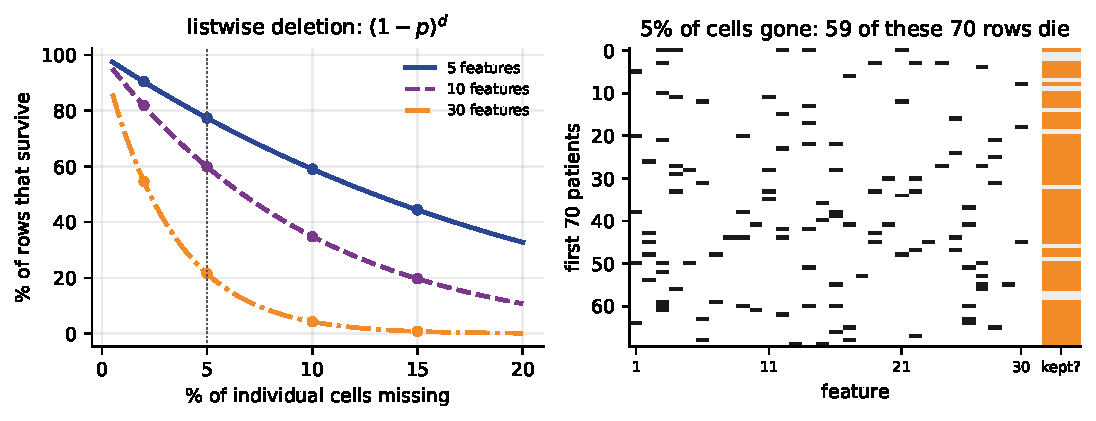
\includegraphics[width=0.84\textwidth]{listwise.pdf}
  \caption{Left: Equation~\eqref{eq:listwise}, drawn, with measured points
  from 200 simulations each. The dotted line is $p = 5\%$. Right: the actual
  missingness mask for the first 70 patients. Black cells are missing; the
  strip on the right is orange if that row is deleted. Fifty-nine of these
  seventy patients die of one missing number.}
  \label{fig:listwise}
\end{figure}

Was it at least safe? On this dataset, more or less --- and it is worth being
honest about that rather than overstating the case.

\begin{codeout}
accuracy on the 114 survivors             0.9735  +/- 0.0216
accuracy imputing instead, all 569 rows   0.9719  +/- 0.0129
baseline with no missingness at all       0.9807  +/- 0.0065
\end{codeout}

Deleting did not lose accuracy here. It lost $455$ patients and produced an
estimate with $1.7$ times the spread. On a harder problem it is not so kind:
Section~\ref{sec:whichimputer} shows the same procedure on
\texttt{load\_diabetes} at $30\%$ missingness leaving \textbf{nine} training
rows for ten features and a model scoring $R^2 = -4.70$.

\begin{keyidea}
Deleting incomplete rows is a decision to throw away evidence, and the amount
you throw away grows exponentially with the number of columns. Sometimes it is
the right decision. It is never the free one.
\end{keyidea}

\notesources{\AMLUnitIVSources}

% =========================================================================
\section{Handling missing data}
\label{sec:missing}

\subsection{Three questions to ask about a hole}

Before you type \texttt{fillna}, answer these.

\textbf{1. Why is it missing?} A sensor failed, a question was refused, a test
was never ordered, a field was added to the form in year three --- four
different problems. \textbf{2. Is the reason related to the value that is
missing?} This is the MCAR / MAR / MNAR question of
Section~\ref{sec:mechanisms}, and it decides whether any imputer can help you
at all. \textbf{3. Is the \emph{fact} of the hole informative?} If a test is
ordered only for patients who already look ill, then ``this value is missing''
predicts the label; Section~\ref{sec:indicator} measures that.

\subsection{Mean, median and mode, by hand}

\begin{worked}[Eight marks, two of them missing]
\[
  55,\ 62,\ ?,\ 71,\ 58,\ ?,\ 90,\ 64
\]
Six values are observed. Sort them: $55,\ 58,\ 62,\ 64,\ 71,\ 90$.

\medskip
\textbf{Mean.} $(55+62+71+58+90+64)/6 = 400/6 = 66.6667$.

\textbf{Median.} With six values it is the average of the third and fourth:
$(62+64)/2 = 63$.

\textbf{Standard deviation}, using the $n-1$ divisor:
$s = \sqrt{\frac{1}{5}\sum(x_i - 66.6667)^2} = 12.6754$.

\medskip
The mean sits $3.67$ marks above the median because of the single $90$. That
gap is the whole reason both statistics exist: the mean uses every value's
distance, the median only its rank.

\medskip
\textbf{Which do you fill with?} \emph{Mean} for a roughly symmetric numeric
column. \emph{Median} when the column is skewed or has outliers, because the
median does not move when a far-away point moves further away. \emph{Mode} ---
the most frequent category --- for a categorical column, where a mean is not
even defined.
\end{worked}

\begin{lstlisting}
marks = np.array([55, 62, np.nan, 71, 58, np.nan, 90, 64])
obs = marks[~np.isnan(marks)]
for name, fill in (("mean", obs.mean()), ("median", np.median(obs))):
    f = np.where(np.isnan(marks), fill, marks)
    print(name, f.mean(), f.std(ddof=1))
\end{lstlisting}
\begin{codeout}
observed values       [55, 62, 71, 58, 90, 64]
n observed 6 of 8
mean of observed         66.6667
median of observed       63.0000
sd of observed (ddof=1)  12.6754
mean   imputed:  mean 66.6667   sd 10.7127   sd is now 84.5% of the truth
median imputed:  mean 65.7500   sd 10.8463   sd is now 85.6% of the truth
\end{codeout}

Two things happened that nobody asked for. The mean-imputed column kept its
mean --- of course, you added copies of the mean --- but its standard deviation
fell by $15.5\%$. The median-imputed column's mean \emph{moved}, from $66.67$
to $65.75$.

\subsection{Mean imputation shrinks the variance, exactly}
\label{sec:shrink}

That $15.5\%$ is not an accident of these eight numbers. It is a theorem.

\begin{worked}[The shrinkage factor]
Let $m$ values be observed out of $n$, with observed mean $\bar x$. Fill the
$n - m$ holes with $\bar x$.

\textbf{The mean cannot move.} The new sum is
$\sum_{i=1}^m x_i + (n-m)\bar x = m\bar x + (n-m)\bar x = n \bar x$, so the new
mean is $\bar x$.

\textbf{The sum of squared deviations cannot move either.} Each new value
contributes $(\bar x - \bar x)^2 = 0$.

So the numerator of the variance is unchanged while the denominator grows:
\begin{equation}
  \label{eq:shrink}
  \sigma^2_{\text{after}}
  = \frac{\sum_{i=1}^{m}(x_i-\bar x)^2}{n}
  = \frac{m}{n}\,\sigma^2_{\text{before}},
  \qquad
  \frac{\sigma_{\text{after}}}{\sigma_{\text{before}}}
  = \sqrt{\frac{m}{n}} = \sqrt{1-p},
\end{equation}
where $p = 1 - m/n$ is the fraction imputed. With the $n-1$ divisor the
corresponding factor is $(m-1)/(n-1)$.

For the eight marks: $m = 6$, $n = 8$, so the population variance is multiplied
by $6/8 = 0.75$ and the sample variance by $5/7 = 0.7143$. The standard
deviation ratio is $\sqrt{0.7143} = 0.8452$, and $10.7127/12.6754 = 0.8452$.
\end{worked}

\begin{codeout}
mean imputation and the variance, exactly
  population variance ratio  m/n         = 0.7500
  sample     variance ratio  (m-1)/(n-1) = 0.7143
  measured, population (ddof=0)          = 0.7500
  measured, sample     (ddof=1)          = 0.7143
\end{codeout}

Now on a real column. Body mass index for the $442$ diabetes patients, in
kg/m$^2$, with the true standard deviation $4.4181$.

\begin{lstlisting}
col = Xr[:, 2]                                  # BMI, original units
rng = np.random.default_rng(0)                  # the one seed for this lecture
for p in (0.1, 0.3, 0.5, 0.7):
    r = []
    for _ in range(2000):
        m = rng.random(len(col)) < p
        v = col.copy()
        v[m] = v[~m].mean()
        r.append(v.std(ddof=1) / col.std(ddof=1))
    print(p, np.mean(r), np.sqrt(1 - p))
\end{lstlisting}
\begin{codeout}
the same law on a real column: diabetes BMI, 2000 draws per row
  p=0.1   measured sd ratio 0.9486   sqrt(1-p) = 0.9487
  p=0.3   measured sd ratio 0.8363   sqrt(1-p) = 0.8367
  p=0.5   measured sd ratio 0.7059   sqrt(1-p) = 0.7071
  p=0.7   measured sd ratio 0.5447   sqrt(1-p) = 0.5477
  largest gap between measurement and sqrt(1-p) here  0.0031
\end{codeout}

Two thousand repetitions per point, and the largest disagreement with
$\sqrt{1-p}$ across the four rows is $0.0031$. Why care? Because everything
you compute afterwards is built out of that standard deviation.

\begin{codeout}
and what that does to a correlation: BMI against the target
  complete data       corr(BMI, y) = 0.5865
  40% mean-imputed    corr(BMI, y) = 0.4538  (77% of it survives)
\end{codeout}

\begin{caution}[Mean imputation manufactures confidence you do not have]
It does not merely lose information --- it \emph{understates} the spread of
the data, so every downstream standard error is too small, every confidence
interval too narrow and every correlation attenuated. A quarter of the
BMI--target correlation disappeared at $40\%$ imputation. Nothing in any
library's output warns you about this, because from the library's point of
view nothing went wrong.
\end{caution}

\begin{figure}[tb]
  \centering
  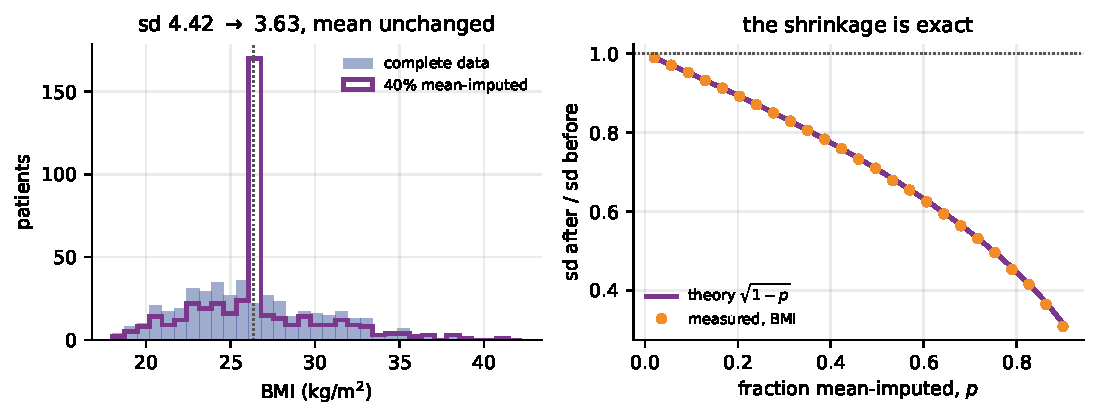
\includegraphics[width=0.84\textwidth]{shrink.pdf}
  \caption{Left: the BMI column before and after mean-imputing it at
  $p = 0.40$. Mean imputation does not blur the distribution --- it piles
  every hidden patient onto one value, and the standard deviation falls from
  $4.4181$ to $3.6309$. This single draw hid $35.29\%$ of the column rather
  than exactly $40\%$, which is why the drop is smaller than $\sqrt{0.6}$
  would suggest; against the $286$ values still observed the shrinkage is
  exact, $0.803902 = \sqrt{285/441}$. Right: the average over $400$ draws per
  point against $\sqrt{1-p}$, which never disagrees by more than $0.0080$.}
  \label{fig:shrink}
\end{figure}

\subsection{MCAR, MAR and MNAR}
\label{sec:mechanisms}

Write $R$ for the indicator that a value is missing, $X_{\text{obs}}$ for the
data you can see and $X_{\text{mis}}$ for the values you cannot. Rubin's
taxonomy asks a single question: \emph{what does $P(R)$ depend on?} The three
answers are named \textbf{MCAR} (missing completely at random), \textbf{MAR}
(missing at random) and \textbf{MNAR} (missing not at random).

\begin{center}
\begin{tabular}{@{}llp{6.4cm}@{}}
\toprule
\textbf{Name} & \textbf{$P(R)$ depends on} & \textbf{Example}\\
\midrule
\textbf{MCAR} & nothing & a tube was dropped in the lab; a page of the
  questionnaire was lost\\[3pt]
\textbf{MAR}  & $X_{\text{obs}}$ only & BMI was recorded only for patients
  flagged with high blood pressure --- and blood pressure \emph{is} in the
  table\\[3pt]
\textbf{MNAR} & $X_{\text{mis}}$ itself & the heaviest patients declined to be
  weighed; the highest earners refused the income question\\
\bottomrule
\end{tabular}
\end{center}

The names are unhelpful --- ``missing at random'' does not mean random --- but
the consequences are sharp. Under \textbf{MCAR} the complete cases are a fair random sample of the whole:
you lose statistical power, not correctness. Under \textbf{MAR} the complete
cases are biased, but the variables that caused the bias are in your table, so
a model that conditions on them can undo it. Under \textbf{MNAR} the
information you would need was never recorded, and \emph{no procedure applied
to the data can fix this} --- you need an external assumption, a sensitivity
analysis, or better data collection.

Construct all three on the same column and measure.

\begin{lstlisting}
bmi, bp = Xr[:, 2], Xr[:, 3]
rng = np.random.default_rng(0)               # the one seed for this lecture
mcar = rng.random(n) < 0.40                  # a coin
mar  = bp < np.median(bp)                    # depends on BP, which we see
mnar = bmi > np.quantile(bmi, 0.60)          # depends on BMI itself
for name, m in (("MCAR", mcar), ("MAR ", mar), ("MNAR", mnar)):
    print(name, bmi[~m].mean(), bmi[~m].mean() - bmi.mean())
\end{lstlisting}
\begin{codeout}
complete-data mean BMI  26.3758 kg/m2   (n = 442)
  MCAR  35.3% missing   complete-case mean 26.4913   bias +0.1155
  MAR   48.0% missing   complete-case mean 27.7230   bias +1.3473
  MNAR  40.0% missing   complete-case mean 23.4253   bias -2.9505
\end{codeout}

Throwing away the incomplete rows costs $+0.12\ \mathrm{kg/m^2}$ under MCAR
--- noise, and it would change sign with another draw --- against $+1.35$
under MAR and $-2.95$ under MNAR. The last of those is two thirds of a
standard deviation, from a decision nobody consciously made.

\begin{figure}[tb]
  \centering
  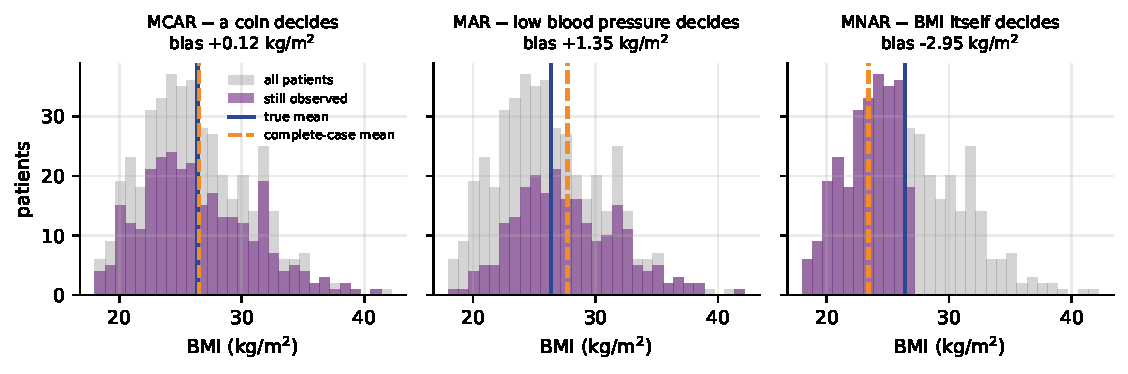
\includegraphics[width=0.88\textwidth]{mechanisms.pdf}
  \caption{Grey is every patient, purple is who is still observed. Under MCAR
  the purple histogram is a shrunken copy of the grey one and the two vertical
  lines coincide. Under MNAR the right tail is simply gone.}
  \label{fig:mechanisms}
\end{figure}

Now the question that makes the taxonomy operational: can a smarter imputer
repair the damage? \texttt{IterativeImputer} --- scikit-learn's version of
MICE --- models each incomplete column as a regression on all the others and
cycles until it settles.

\begin{lstlisting}
from sklearn.experimental import enable_iterative_imputer   # required
from sklearn.impute import SimpleImputer, IterativeImputer
for name, m in mech.items():
    Z = Xr.copy(); Z[m, 2] = np.nan
    for label, imp in (("mean", SimpleImputer(strategy="mean")),
                       ("MICE", IterativeImputer(random_state=0,
                                                 max_iter=30))):
        print(name, label, imp.fit_transform(Z)[:, 2].mean())
\end{lstlisting}
\begin{codeout}
can an imputer that uses the other columns repair it?
  MCAR mean     imputed mean 26.4913   bias +0.1155
  MCAR MICE     imputed mean 26.4763   bias +0.1005
  MAR  mean     imputed mean 27.7230   bias +1.3473
  MAR  MICE     imputed mean 26.2170   bias -0.1588
  MNAR mean     imputed mean 23.4253   bias -2.9505
  MNAR MICE     imputed mean 23.7924   bias -2.5834
\end{codeout}

Read the middle pair. Under MAR, MICE cut the bias from $+1.3473$ to $-0.1588$
--- a factor of $8.5$ --- because blood pressure was recorded and BMI can be
predicted from it. Read the last pair. Under MNAR it moved $-2.9505$ to
$-2.5834$ and stopped, because the patients it needed to learn from are not in
the file.

\begin{keyidea}
The mechanism decides what is possible. MCAR: lose power, keep correctness.
MAR: a multivariate imputer can recover the truth, and here it recovered
$88\%$ of the bias. MNAR: nothing in the data can help, and pretending
otherwise is how a wrong number gets published.
\end{keyidea}

It gets worse than a shifted mean. Fit a linear regression of disease
progression on all ten features and read off the BMI coefficient.

\begin{codeout}
and what the MNAR column does to a fitted coefficient
  true BMI coefficient             5.603
  MNAR + mean imputation          -0.413
  MNAR + MICE                      2.299
\end{codeout}

\begin{caution}[The sign flipped]
Mean-imputing an MNAR column replaced the entire upper $40\%$ of the BMI
distribution with a single constant. The slope fitted through what remained
points the \emph{other way}: $+5.603$ became $-0.413$. Written up, that reads
``BMI is not associated with disease progression'', which is the opposite of
the truth. Prediction is more forgiving than inference, but only because
nobody reads a predictor's coefficients.
\end{caution}

\subsection{So which imputer should you actually use?}
\label{sec:whichimputer}

The honest experiment: hold out a clean test set, punch MCAR holes in the
\emph{training} matrix only, and compare seven strategies over twenty random
splits.

\begin{lstlisting}
for seed in range(0, 20):        # a sweep: the spread over splits is the point
    Xtr, Xte, ytr, yte = train_test_split(Xd, yd, test_size=0.25,
                                          random_state=seed)
    Xm = Xtr.copy()
    Xm[np.random.default_rng(100 + seed).random(Xtr.shape) < p] = np.nan
    mdl = make_pipeline(imputer, LinearRegression()).fit(Xm, ytr)
    score = mdl.score(Xte, yte)
\end{lstlisting}
\begin{codeout}
diabetes, 10% of TRAIN cells missing (MCAR), clean test set, 20 splits
  oracle, no missingness   test R2 0.4762  +/- 0.0506
  drop incomplete rows     test R2 0.4264  +/- 0.0630
  mean                     test R2 0.4721  +/- 0.0548
  median                   test R2 0.4727  +/- 0.0544
  constant 0               test R2 0.4723  +/- 0.0548
  KNN, k=5                 test R2 0.4743  +/- 0.0527
  iterative (MICE)         test R2 0.4751  +/- 0.0505
  rows surviving listwise deletion 114 of 331   (1-p)**10 = 0.349
\end{codeout}
\begin{codeout}
diabetes, 30% of TRAIN cells missing (MCAR), clean test set, 20 splits
  oracle, no missingness   test R2 0.4762  +/- 0.0506
  drop incomplete rows     test R2 -4.6952  +/- 7.8838
  mean                     test R2 0.4351  +/- 0.0697
  median                   test R2 0.4364  +/- 0.0698
  constant 0               test R2 0.4365  +/- 0.0690
  KNN, k=5                 test R2 0.4591  +/- 0.0580
  iterative (MICE)         test R2 0.2639  +/- 0.5004
  rows surviving listwise deletion 9 of 331   (1-p)**10 = 0.028
\end{codeout}

Three readings, in order of importance.

\textbf{Dropping rows is expensive and everything else is cheap.} At $10\%$
missingness the five imputers span $0.4721$ to $0.4751$ --- three thousandths
of $R^2$ --- and all sit within $0.004$ of the oracle that never lost any data.
Deletion costs $0.05$. At $30\%$ it leaves nine rows for ten features and the
fit is worse than predicting the mean.

\textbf{At heavy missingness a multivariate imputer earns its keep}: KNN at
$30\%$ recovers $0.4591$ against mean imputation's $0.4351$.

\textbf{And be honest about MICE.} Its $30\%$ entry is $0.2639 \pm 0.5004$ ---
a standard deviation ten times any other row's --- because on two of the twenty
splits the round-robin regressions produced nearly collinear imputed columns
and the least-squares fit blew up. Bounding with \texttt{min\_value} and
\texttt{max\_value} reduced this but did not eliminate it.

\begin{figure}[tb]
  \centering
  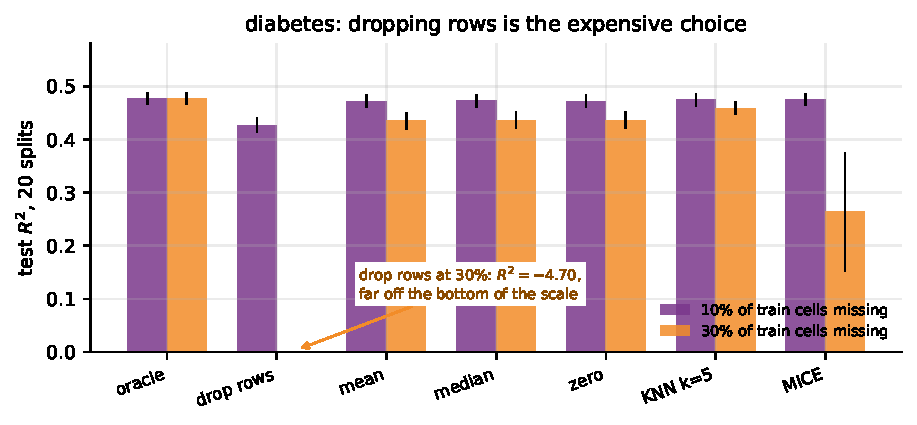
\includegraphics[width=0.70\textwidth]{imputescores.pdf}
  \caption{The two tables above, drawn. Error bars are standard errors over
  twenty splits. Six of the seven bars are the same height; the one that is
  not is the one most people reach for first.}
  \label{fig:imputescores}
\end{figure}

\begin{keyidea}
Do not agonise over which imputer. Do agonise over whether you are deleting
rows. On these measurements the gap between the best and worst imputer was
$0.003$ of $R^2$ and the gap between imputing and deleting was $0.05$ --- and
at $30\%$ missingness, $5.1$.
\end{keyidea}

\subsection{Missingness is itself data}
\label{sec:indicator}

Sometimes the most informative thing about a value is that it is not there. A
diagnostic test that is only ordered when a clinician already suspects
something will be missing for the healthy patients. Then ``missing'' predicts
the label directly, and imputing it away destroys that.

\begin{lstlisting}
SimpleImputer(strategy="mean", add_indicator=True)
\end{lstlisting}
\begin{codeout}
one weak feature, missing 80% of the time for class 1, 20% for class 0
  mean imputation only          0.6294
  mean imputation + indicator   0.7969
  difference                   +0.1675
\end{codeout}

Sixteen and a half points, from a column of booleans and one keyword argument.

\begin{caution}[And the same feature can be leakage]
The indicator is legitimate only if the reason for the hole will still exist
when the model is deployed. If the test was skipped because the outcome was
already known --- a diagnosis recorded before the test was ordered --- then
you have encoded the answer into the features, and your test accuracy is
measuring your data collection process rather than your model. Ask
\emph{when}, in the real timeline, the missingness is decided.
\end{caution}

\begin{tryit}
Impute the eight marks with
\texttt{SimpleImputer(strategy="most\_frequent")}. All six observed values are
distinct, so the mode is not unique: predict what scikit-learn does, then check
(it takes the smallest, $55$).
\end{tryit}

% =========================================================================
\section{Describing the shape of a column}
\label{sec:shape}

Everything so far has used two numbers to describe a column: a centre and a
spread. They are the first two moments, and between them they tell you nothing
about \emph{shape}. Two columns can share a mean and a standard deviation to
four decimals and still look nothing alike --- one symmetric and tame, the
other with a tail running off to the right that will decide every choice you
make in the next two sections.

The next two numbers up the ladder fix that. \textbf{Skewness} asks which side
the tail is on. \textbf{Kurtosis} asks how much of the data is out in the tails
at all. You need both before you can choose between a mean and a median, before
you can read an outlier rule honestly, and before you can tell whether a
transformation has done anything.

\subsection{The moments, and the two shape statistics}

Write $d_i = x_i - \bar{x}$ for the deviation of each observation from the
mean. The \emph{$k$th central moment} is the average $k$th power of those
deviations:

\begin{equation}
  m_k \;=\; \frac{1}{n}\sum_{i=1}^{n} d_i^{\,k}
  \;=\; \frac{1}{n}\sum_{i=1}^{n} (x_i - \bar{x})^k .
  \label{eq:moment}
\end{equation}

$m_1$ is zero by construction. $m_2$ is the variance. The two shape statistics
are the next two moments, each divided by the right power of the standard
deviation so that the answer is a pure number:

\begin{equation}
  \underbrace{g_1 = \frac{m_3}{m_2^{3/2}}}_{\text{skewness}}
  \qquad\qquad
  \underbrace{b_2 = \frac{m_4}{m_2^{2}}}_{\text{kurtosis}}
  \qquad\qquad
  \underbrace{g_2 = b_2 - 3}_{\text{excess kurtosis}} .
  \label{eq:shape}
\end{equation}

That division is what makes them useful. Measure a column in millimetres
instead of metres and the mean, the variance and every moment change; $g_1$ and
$b_2$ do not move at all. They describe shape and nothing else.

\begin{keyidea}[What the two numbers ask]
Skewness is an \textbf{odd} power, so the sign of a deviation survives and one
long tail fails to cancel: $g_1 > 0$ means the tail runs right, $g_1 < 0$ means
it runs left, $g_1 = 0$ means the two sides balance.

Kurtosis is an \textbf{even} power, so sign is destroyed and only magnitude
counts --- and the fourth power weights a deviation of $4$ standard deviations
$256$ times as heavily as one of $1$. It is therefore a statement about the
tails, not about the middle.
\end{keyidea}

The $-3$ in the excess kurtosis is a convention, not mathematics. A normal
distribution has $b_2 = 3$ exactly, so subtracting $3$ puts the normal at zero
and lets you read the sign as ``heavier tails than a normal'' or ``lighter''.
Both conventions are in use and confusing them is the most common error in this
material: \texttt{scipy.stats.kurtosis} returns the \emph{excess} form by
default, while many textbooks and spreadsheet functions report $b_2$ itself.

\begin{worked}[Both statistics on five numbers, by hand]
Take $x = (1, 2, 2, 3, 7)$, chosen so the mean is a whole number. Then
$\bar{x} = 3$ and the deviations are $(-2, -1, -1, 0, 4)$.

\medskip
\begin{tabular}{@{}lll@{}}
\toprule
moment & sum of powers & value\\
\midrule
$m_2$ & $(4 + 1 + 1 + 0 + 16)/5$   & $22/5 = 4.4$\\
$m_3$ & $(-8 - 1 - 1 + 0 + 64)/5$  & $54/5 = 10.8$\\
$m_4$ & $(16 + 1 + 1 + 0 + 256)/5$ & $274/5 = 54.8$\\
\bottomrule
\end{tabular}

\medskip
Notice where each total comes from. In $m_3$ the single value $7$ contributes
$+64$ against $-10$ from everything else combined, so one point decides the
sign. In $m_4$ it contributes $256$ of the $274$ --- \textbf{93\% of the
total from one observation in five}.

\[
  g_1 = \frac{10.8}{4.4^{3/2}} = \frac{10.8}{9.2295} = +1.1702,
  \qquad
  b_2 = \frac{54.8}{4.4^{2}} = \frac{54.8}{19.36} = 2.8306,
\]
so the excess kurtosis is $2.8306 - 3 = -0.1694$.

The skewness is clearly positive, as the picture demands. The excess kurtosis
is \emph{negative} despite the obvious outlier, which looks wrong and is not
--- see Section~\ref{sec:shapeceiling}.
\end{worked}

\begin{lstlisting}
x = np.array([1.0, 2.0, 2.0, 3.0, 7.0])
d = x - x.mean()
m2, m3, m4 = (d**2).mean(), (d**3).mean(), (d**4).mean()
print("g1 =", m3 / m2**1.5, "  b2 =", m4 / m2**2)
print("scipy:", stats.skew(x), stats.kurtosis(x), stats.kurtosis(x, fisher=False))
\end{lstlisting}
\begin{codeout}
x    = [1. 2. 2. 3. 7.]
mean = 3.0000   deviations = [-2. -1. -1.  0.  4.]
m2 = mean(d^2) = 4.4000
m3 = mean(d^3) = 10.8000
m4 = mean(d^4) = 54.8000

skewness g1 = m3 / m2^1.5 = 10.8000 / 9.2295 = +1.1702
kurtosis b2 = m4 / m2^2   = 54.8000 / 19.3600 = +2.8306
excess      = b2 - 3      = -0.1694

scipy:  skew +1.1702   kurtosis -0.1694 (excess)   +2.8306 (Pearson)
\end{codeout}

\subsection{Two corrections scipy applies, and when they matter}

Equation~\eqref{eq:shape} divides by $n$. Those are the \emph{population}
moments applied to a sample, and like the $1/n$ variance they are biased
downwards. The bias-corrected versions, written $G_1$ and $G_2$, rescale them:

\begin{equation}
  G_1 \;=\; \frac{\sqrt{n(n-1)}}{n-2}\; g_1 .
  \label{eq:G1}
\end{equation}

\begin{lstlisting}
print(stats.skew(x), stats.skew(x, bias=False))
print(stats.kurtosis(x), stats.kurtosis(x, bias=False))
\end{lstlisting}
\begin{codeout}
scipy reports the biased estimator unless you ask otherwise.
                biased     bias-corrected
skewness        +1.1702        +1.7444
excess kurt     -0.1694        +3.3223
G1 = sqrt(n(n-1))/(n-2) * g1 = 1.4907 * +1.1702 = +1.7444
the factor is 1.4907 at n=5, 1.0534 at n=30, 1.0030 at n=500 -- it matters
only on small samples, which is where the estimate is worthless anyway
\end{codeout}

At $n = 5$ the correction inflates the skewness by half again and flips the
excess kurtosis from $-0.17$ to $+3.32$. At $n = 500$ it changes the third
decimal. That last line is the honest summary: the correction is largest
exactly where the estimate is too noisy to act on, so it rarely rescues a
decision. What it does do is guarantee that two people analysing the same
column disagree unless they say which convention they used.

\begin{caution}[Always say which convention you are quoting]
``Kurtosis $3.3$'' is ambiguous three ways: Pearson or excess, biased or
corrected, and --- in a spreadsheet --- possibly a fourth definition again.
Quote the library call, not the number alone. In this course, every kurtosis is
\texttt{scipy.stats.kurtosis} with its defaults: \textbf{excess, biased}.
\end{caution}

\subsection{What the values look like for familiar distributions}

\begin{lstlisting}
for name, v in families:              # 200,000 draws each, seed 0
    print(name, stats.skew(v), stats.kurtosis(v))
\end{lstlisting}
\begin{codeout}
distribution     skewness  excess kurt
normal            -0.0036      +0.0079
uniform           +0.0029      -1.2002
Student t, 5      -0.0090      +4.6239
left-skewed       -1.9953      +5.9772
exponential       +2.0025      +6.0578
lognormal         +6.0346     +86.4337

theory: normal 0, 0   uniform 0, -1.2   exponential +2, +6
\end{codeout}

\begin{figure}[htbp]
  \centering
  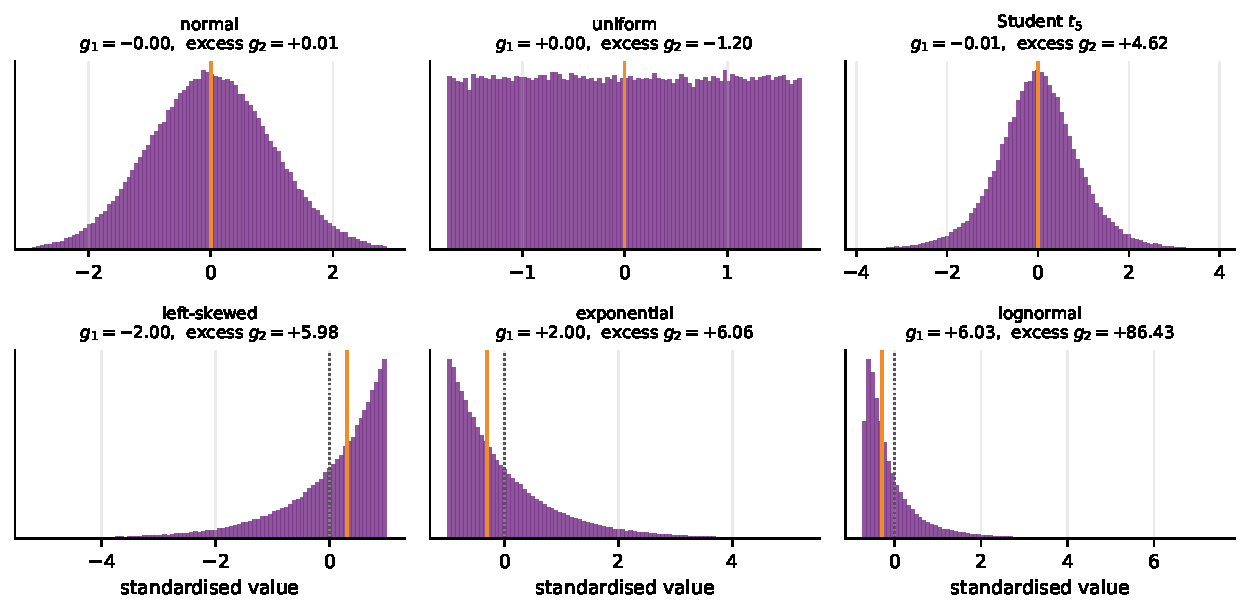
\includegraphics[width=\textwidth]{../figures/shape.pdf}
  \caption{Six distributions, each standardised, with its two shape numbers.
  The dotted line is the mean and the orange line the median; the gap between
  them opens as the skewness grows. The normal and the uniform are both
  perfectly symmetric and differ only in kurtosis: the uniform has no tails at
  all, which is what a negative excess kurtosis means.}
  \label{fig:shape}
\end{figure}

Three of those are exact theoretical values and the sample estimates land on
them, which is the check that the code is doing what the algebra says. The
uniform is the useful case to remember: perfectly symmetric, so $g_1 = 0$, but
$g_2 = -1.2$ because it stops dead at its limits and has no tails to speak of.
Negative excess kurtosis is not a defect, it is a bounded variable.

\subsection{Kurtosis measures the tails, not the peak}
\label{sec:tailshare}

Many textbooks describe kurtosis as ``peakedness''. That is at best misleading,
and it is worth one experiment to see why. Compare a standard normal with a
\emph{scale mixture}: 95\% of the values drawn with standard deviation $0.8$
and 5\% with standard deviation $3.0$, then standardised so both columns have
standard deviation exactly $1$.

\begin{lstlisting}
d4 = (v - v.mean())**4
tail = np.abs(v) > 3
print(tail.mean(), d4[tail].sum() / d4.sum(), stats.kurtosis(v))
\end{lstlisting}
\begin{codeout}
                density at 0     % |z|>3    excess kurt   share of sum d^4
normal                0.4002      0.2830         0.0079             0.1134
95/5 mixture          0.4941      1.5005         9.0433             0.8761

The mixture is taller at the centre AND heavier in the tails; both are
true.  The decomposition settles which one the statistic is counting:
1.50% of its rows supply 88% of the fourth-power sum.
\end{codeout}

The mixture \emph{is} about a quarter taller at the centre, so the ``peakedness''
story is not simply false --- the two features usually travel together, because
standardising a column with heavy tails inflates its standard deviation and
squeezes the middle upwards. But the decomposition settles which one the
statistic is actually counting. Split $\sum d_i^4$ into the part contributed by
rows beyond $\pm 3$ and the rest: in the mixture, \textbf{1.5\% of the rows
supply 88\% of the sum}. The peak contributes almost nothing, because small
deviations raised to the fourth power are negligible.

\begin{keyidea}[Read kurtosis as an outlier-frequency statistic]
High kurtosis says: this column produces extreme values more often than a
normal distribution would. That is a statement about how often your outlier
rule will fire, which is why this section sits immediately before the one on
outliers.
\end{keyidea}

\subsection{Both estimates are noisy, and the thresholds are folklore}

You will find rules of thumb --- $|g_1| < 0.5$ is ``fairly symmetric'',
$|g_1| > 1$ is ``highly skewed'', $|g_2| > 3$ is ``heavy-tailed''. Before
using any of them, look at how much these statistics move on data that has no
skew at all.

\begin{lstlisting}
for n in (20, 30, 100, 1000):         # 1000 samples of a standard normal
    sk = [stats.skew(rng(i).standard_normal(n)) for i in range(1000)]
    print(n, np.mean(sk), np.std(sk), np.sqrt(6 / n))
\end{lstlisting}
\begin{codeout}
1000 samples from a standard normal, where both true values are 0:
     n    mean skew    sd skew      sqrt(6/n)   sd exc k
    20      -0.0387     0.4567         0.5477     0.7289
    30      -0.0223     0.3932         0.4472     0.6891
   100      -0.0037     0.2394         0.2449     0.4468
  1000      +0.0032     0.0787         0.0775     0.1531

at n=30, 20.4% of samples from a perfectly symmetric distribution
report |skewness| > 0.5, the threshold often quoted as 'skewed'
\end{codeout}

The standard errors are approximately $\sqrt{6/n}$ for skewness and
$\sqrt{24/n}$ for excess kurtosis, and the measured spreads sit right on those
values. The consequence is stark: at $n = 30$, \textbf{one sample in five}
drawn from a perfectly symmetric distribution crosses the threshold that would
have you declare the column skewed and reach for a transformation.

\begin{caution}[A shape statistic on a small column is not evidence]
At $n = 30$ the standard error of the skewness is $0.45$. A reported value of
$0.6$ is less than one and a half standard errors from zero --- it is
indistinguishable from symmetry. Use these numbers on columns of a few hundred
rows and up, use the figures at every size, and never transform a column
because a statistic computed on thirty values crossed a threshold somebody
wrote in a textbook.
\end{caution}

\begin{figure}[htbp]
  \centering
  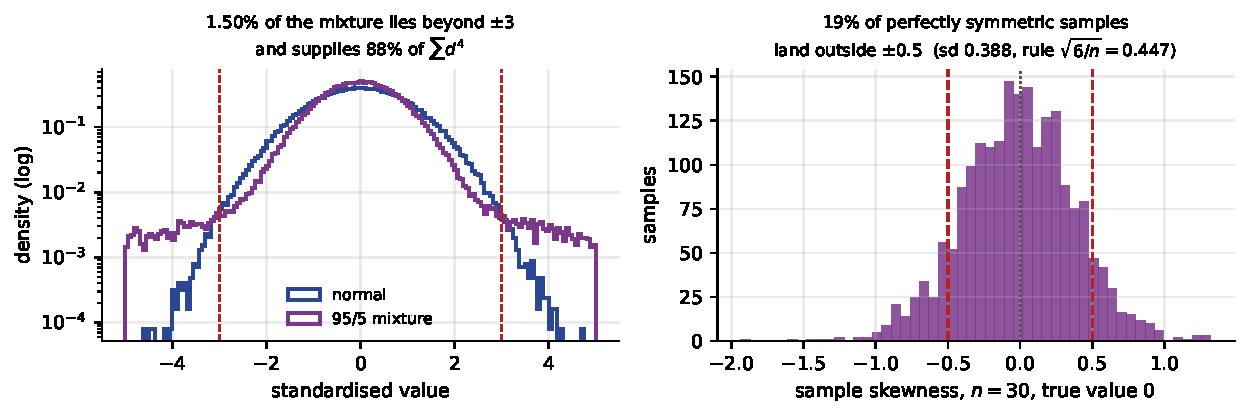
\includegraphics[width=\textwidth]{../figures/tailshare.pdf}
  \caption{Left: the two columns on a log density scale, with the share of
  $\sum d^4$ contributed from beyond $\pm 3$ marked --- the mixture's tail is
  a rounding error in the row count and almost all of the statistic. Right: the
  sampling distribution of skewness at $n = 30$ under perfect symmetry, against
  the $\pm 0.5$ threshold quoted as if it described the data.}
  \label{fig:tailshare}
\end{figure}

\subsection{Both statistics have a ceiling that depends only on \texorpdfstring{$n$}{n}}
\label{sec:shapeceiling}

This is why the five-point example returned a negative excess kurtosis while
staring at an obvious outlier. Exactly as the $z$-score has an algebraic
ceiling of $(n-1)/\sqrt{n}$ (Section~\ref{sec:ceiling}), so do both shape
statistics:

\begin{equation}
  |g_1| \;\le\; \frac{n-2}{\sqrt{n-1}},
  \qquad\qquad
  b_2 \;\le\; \frac{n^2 - 3n + 3}{n - 1}.
  \label{eq:shapebound}
\end{equation}

\begin{codeout}
     n    one outlier   best 2-point split   (n^2-3n+3)/(n-1) - 3
     5         0.2500               0.2500                 0.2500
    10         5.1111               5.1111                 5.1111
    30        25.0345              25.0345                25.0345
   100        95.0101              95.0101                95.0101
   569       564.0018             564.0018               564.0018

All three agree to every digit.  The tight bound is
    b2 <= (n^2 - 3n + 3)/(n - 1),   attained by one point standing
away from n-1 equal ones -- exactly what a single gross outlier does.
Skewness is bounded the same way by |g1| <= (n-2)/sqrt(n-1):
    n=  5  measured   1.5000  bound   1.5000
    n= 30  measured   5.1995  bound   5.1995
    n=569  measured  23.7908  bound  23.7908
\end{codeout}

At $n = 5$ the largest excess kurtosis any five numbers can produce is
$\mathbf{0.25}$. Our example returned $-0.17$, which is most of the way to the
maximum --- it was not saying ``light tails'', it was saying ``as heavy as five
points are allowed to be''. The bound is tight and is attained by precisely the
configuration a single gross outlier creates: one point standing away from
$n-1$ equal ones. The looser $n-3$ you will sometimes see quoted is never
reached.

\begin{caution}[A small kurtosis on a short column means nothing]
Below about fifty rows, both statistics are squeezed between a hard ceiling and
a standard error of their own size. Plot the column. The histogram has no such
limitation and you will see in one second what the statistic cannot tell you.
\end{caution}

\subsection{Why this decides the choices in the next two sections}

The point of this section is not the formulas, it is that the two numbers
change what you do.

\begin{lstlisting}
for name in ("mean radius", "mean texture", "area error", "worst area"):
    v = bc.data[:, list(bc.feature_names).index(name)]
    print(name, stats.skew(v), stats.kurtosis(v), v.mean(), np.median(v))
\end{lstlisting}
\begin{codeout}
column            skew     exc k       mean     median     gap %
mean radius     +0.940     +0.83     14.127     13.370      5.7%
mean texture    +0.649     +0.74     19.290     18.840      2.4%
area error      +5.433    +48.77     40.337     24.530      64.4%
worst area      +1.854     +4.35    880.583    686.500      28.3%

the more skewed the column, the further the mean sits from the median,
and the worse an imputed mean represents a typical row
\end{codeout}

\begin{itemize}
  \item \textbf{Which imputer.} The skewness tells you how far apart the mean
    and the median are, and therefore how much damage mean imputation does. On
    \texttt{mean texture}, at $g_1 = 0.65$, they differ by 2.4\% and the choice
    hardly matters. On \texttt{area error}, at $g_1 = 5.43$, the mean sits
    \textbf{64\% above the median} and only 28.6\% of rows are above it ---
    filling holes with the mean inserts a value more extreme than seven rows in
    ten.
  \item \textbf{How to read an outlier rule.} The kurtosis predicts how often
    a $z$-score or IQR rule will fire. On \texttt{area error}, $g_2 = 48.8$
    guarantees a lot of flagged rows, and Section~\ref{sec:skewrules} shows
    they are not contamination --- the rule is detecting the shape you have
    just measured.
  \item \textbf{Whether a transformation worked.} Both numbers give you a
    target to check against, which is exactly how Section~\ref{sec:boxcox}
    reports its results.
\end{itemize}

\begin{tryit}
Compute both statistics for every column of \texttt{load\_breast\_cancer}, then
sort by skewness. Look at the histogram of the most skewed column and the least
skewed one. Then check the claim in the paragraph above: is the share of rows
above the mean close to $0.5$ for the symmetric column, and well below it for
the skewed one?
\end{tryit}

% =========================================================================
\section{Handling outliers}
\label{sec:outliers}

\subsection{Three kinds of outlier and one word for all of them}

An outlier is an observation that deviates markedly from the others. That
definition says nothing about what to do, because there are three completely
different things it can be. \textbf{An error} --- an age of $200$, a blood
pressure in the wrong units, a sensor stuck at its rail voltage: fix it or
remove it. \textbf{A rare truth} --- a genuinely enormous tumour or salary:
keep it, and use a method that is not destroyed by it. \textbf{The point of
the exercise} --- fraud, a failing machine, a novel astronomical object: it is
the signal, not the noise.

\begin{keyidea}
No statistical rule can distinguish these three. A rule tells you a point is
unusual; only knowledge of where the data came from tells you what it means.
Detection is statistics; disposal is a judgement you must be able to defend in
writing.
\end{keyidea}

Iglewicz and Hoaglin, whose 1993 monograph is the standard reference and the
source of the modified $z$-score below, separate three activities:
\emph{labelling} (flag candidates for investigation), \emph{accommodation}
(use a method robust enough not to care) and \emph{identification} (formally
test whether a point is an outlier). Most of what follows is labelling, which
is what a preprocessing pipeline actually needs.

\subsection{Three rules}
\label{sec:rules}

\begin{align}
  \text{$z$-score:}\quad & z_i = \frac{x_i - \bar x}{s},
    && \text{flag if } |z_i| > 3, \label{eq:zrule}\\[3pt]
  \text{Tukey fence:}\quad & \mathrm{IQR} = Q_3 - Q_1,
    && \text{flag if } x_i < Q_1 - 1.5\,\mathrm{IQR}
       \text{ or } x_i > Q_3 + 1.5\,\mathrm{IQR}, \label{eq:iqrrule}\\[3pt]
  \text{modified $z$:}\quad & M_i = \frac{0.6745\,(x_i - \tilde x)}{\mathrm{MAD}},
    && \text{flag if } |M_i| > 3.5. \label{eq:mzrule}
\end{align}

Here $\tilde x$ is the median and
$\mathrm{MAD} = \operatorname{median}_i |x_i - \tilde x|$ is the \emph{median
absolute deviation}. Three constants need explaining.

\textbf{Why $0.6745$}: for Normal data $\mathrm{MAD} \approx 0.6745\,\sigma$,
because $0.6745$ is the $0.75$ quantile of the standard Normal, so dividing by
it puts $M$ back on the $z$ scale. \textbf{Why $1.5$}: for Normal data
$Q_3 + 1.5\,\mathrm{IQR}$ sits at about $2.70\sigma$, so the fence flags
$0.70\%$ of observations; Tukey chose it as a convenient round number, not by
derivation. \textbf{Why $3$ and $3.5$}: $|z| > 3$ flags $0.27\%$ of Normal
data, and Iglewicz and Hoaglin recommend $3.5$ for the modified score.

The important column below is the last. The \textbf{breakdown point} of an
estimator is the fraction of the sample you must corrupt before you can move
the estimate arbitrarily far.

\begin{center}
\begin{tabular}{@{}llp{5.6cm}@{}}
\toprule
\textbf{Rule} & \textbf{Breakdown point} & \textbf{Why}\\
\midrule
$z$-score    & $0\%$  & one observation can move $\bar x$ and $s$ as far as
                        you like\\
Tukey / IQR  & $25\%$ & the quartiles do not move until you corrupt a quarter
                        of the data\\
modified $z$ & $50\%$ & both the median and the MAD are medians\\
\bottomrule
\end{tabular}
\end{center}

A breakdown point of $0\%$ is not a technicality. It is the whole of the next
subsection.

\subsection{The rule that cannot see the outlier in front of it}
\label{sec:masking}

\begin{worked}[Thirty-five readings from one sensor]
Thirty genuine readings scattered around $10.0$ with a spread of about $1$,
then the sensor sticks and reports exactly $100.0$ five times. Nobody looking
at this data could miss the problem.

The summary statistics of all thirty-five values:
\begin{center}
\begin{tabular}{@{}lrlr@{}}
\toprule
mean $\bar x$ & $22.503$ & median $\tilde x$ & $9.950$\\
sd $s$        & $32.109$ & MAD               & $0.540$\\
$Q_1$         & $9.245$  & $Q_3$             & $10.330$\\
\bottomrule
\end{tabular}
\end{center}

Now score one stuck reading, $x = 100$, with each rule.

\medskip
\textbf{$z$-score.} $z = (100 - 22.503)/32.109 = 2.4135$. The threshold is $3$.
\textbf{Not flagged.}

\textbf{Tukey fence.} $\mathrm{IQR} = 10.330 - 9.245 = 1.085$, so the upper
fence is $10.330 + 1.5(1.085) = 11.957$. Since $100 > 11.957$: \textbf{flagged}.

\textbf{Modified $z$.} $M = 0.6745(100 - 9.950)/0.540 = 112.48$ against a
threshold of $3.5$. \textbf{Flagged, by a factor of thirty-two.}

\medskip
Why did the first rule fail? The five stuck readings dragged the mean from
$9.586$ up to $22.503$ and inflated the standard deviation from $0.837$ to
$32.109$. \textbf{They are being measured against a ruler that they themselves
bent.} Remove them and recompute: the same reading of $100$ would then score
$z = (100 - 9.586)/0.837 = 108.1$.
\end{worked}

\begin{lstlisting}
z   = (v - v.mean()) / v.std(ddof=1)
q1, q3 = np.percentile(v, [25, 75]);  iqr = q3 - q1
mad = np.median(np.abs(v - np.median(v)))
mz  = 0.6745 * (v - np.median(v)) / mad
\end{lstlisting}
\begin{codeout}
35 readings: 30 genuine near 10.0, then 5 stuck at 100.0
  mean 22.503   sd 32.109   median 9.950   MAD 0.540
  Q1 9.245  Q3 10.330  IQR 1.085  upper fence Q3+1.5*IQR 11.957
  a stuck reading:  z = 2.4135  (needs > 3)   modified z = 112.48  (needs > 3.5)
rule                     flags   of which stuck   of which genuine
  |z| > 3                  0          0               0
  outside 1.5*IQR fence    6          5               1
  |modified z| > 3.5       5          5               0
sd WITHOUT the five stuck readings  0.837
z of a stuck reading would then be  108.1
\end{codeout}

The $z$-score rule found \textbf{none} of the five. The IQR fence found all
five plus one genuine reading (a false positive, which is what a $0.70\%$
Normal-data rate looks like on thirty points). The modified $z$ found exactly
the five.

\begin{caution}[Masking]
This failure has a name. \textbf{Masking} is when the presence of one outlier
prevents another from being detected, because the outliers between them
inflate the very dispersion estimate they are being compared against. Its
mirror image is \textbf{swamping}, where a genuine outlier drags the statistics
far enough that innocent points get flagged too. NIST's handbook singles out
masking as the reason you cannot apply a single-outlier test repeatedly and
expect to find several.
\end{caution}

Masking gets monotonically worse as contamination grows. Add stuck readings one
at a time to the same thirty genuine ones and watch the largest $|z|$ in the
sample:

\begin{codeout}
    k= 0 stuck readings: largest |z|  2.518   largest mod. z     3.3
    k= 1 stuck readings: largest |z|  5.381   largest mod. z   119.3
    k= 2 stuck readings: largest |z|  3.809   largest mod. z   121.7
    k= 3 stuck readings: largest |z|  3.113   largest mod. z   124.1
    k= 4 stuck readings: largest |z|  2.697   largest mod. z   124.1
    k= 5 stuck readings: largest |z|  2.414   largest mod. z   112.5
    k=10 stuck readings: largest |z|  1.710   largest mod. z    76.3
\end{codeout}

One outlier is caught easily at $z = 5.38$. Two are caught at $3.81$, three
barely at $3.11$, and from the fourth onwards the rule never fires again --- no
matter how many more you add. The modified $z$ stays above $60$ throughout.

\begin{figure}[tb]
  \centering
  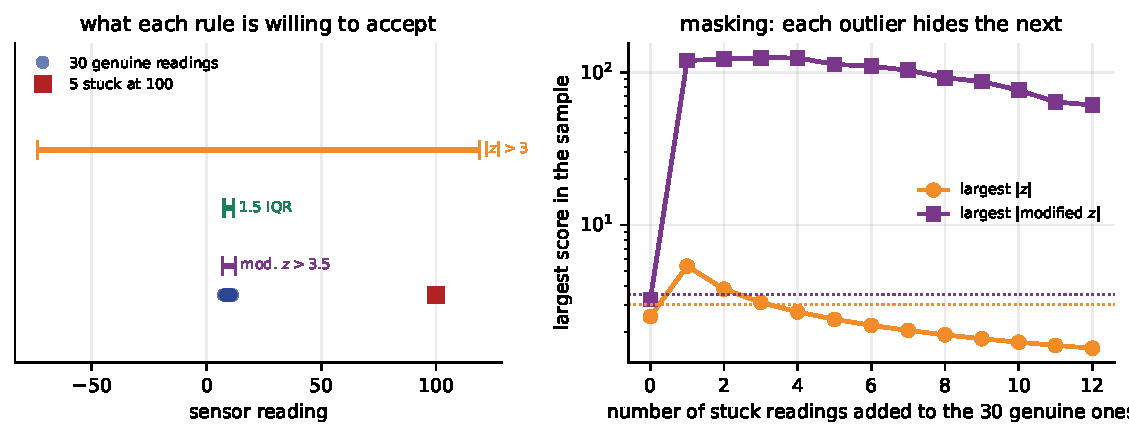
\includegraphics[width=0.88\textwidth]{masking.pdf}
  \caption{Left: the interval of values each rule is willing to accept. The
  $z$ interval runs from $-74$ to $+119$ and comfortably contains the stuck
  readings at $100$; the other two are slivers around $10$. Right: the largest
  score in the sample as stuck readings are added, log scale, with the two
  thresholds dotted.}
  \label{fig:masking}
\end{figure}

\subsection{The rule also has a ceiling}
\label{sec:ceiling}

There is a second, sharper way in which $|z| > 3$ fails, and it does not need
any contamination at all.

\begin{worked}[The maximum attainable $z$-score]
Take any sample of $n$ values with sample standard deviation $s$ (the $n-1$
one). Write $d_i = x_i - \bar x$, so $\sum_i d_i = 0$ and
$\sum_i d_i^2 = (n-1)s^2$.

Suppose $x_1$ is the extreme point. The remaining $n-1$ deviations sum to
$-d_1$, and among all vectors with a fixed sum the sum of squares is smallest
when they are all equal, so
\[
  \sum_{i \ge 2} d_i^2 \;\ge\; (n-1)\left(\frac{-d_1}{n-1}\right)^2
  = \frac{d_1^2}{n-1}.
\]
Therefore
\[
  (n-1)s^2 = d_1^2 + \sum_{i\ge2} d_i^2
  \;\ge\; d_1^2\left(1 + \frac{1}{n-1}\right)
  = d_1^2\,\frac{n}{n-1},
\]
which rearranges to
\begin{equation}
  \label{eq:zmax}
  |z_1| = \frac{|d_1|}{s} \;\le\; \frac{n-1}{\sqrt{n}} .
\end{equation}
Equality holds exactly when the other $n-1$ values are all identical --- the
most extreme possible outlier.
\end{worked}

\begin{codeout}
 n   largest possible |z|   can the rule |z| > 3 ever fire?
  3        1.1547              NO -- not ever
  5        1.7889              NO -- not ever
  8        2.4749              NO -- not ever
 10        2.8460              NO -- not ever
 11        3.0151              yes
 20        4.2485              yes
 50        6.9296              yes
closed form (n-1)/sqrt(n):  n=10 -> 2.8460,  n=11 -> 3.0151
\end{codeout}

\begin{caution}[Below $n = 11$ the rule is not strict, it is inert]
$9/\sqrt{10} = 2.846 < 3$. If you have ten measurements and you write
\texttt{if abs(z) > 3}, you have written a line of code whose value is
\texttt{False} for every possible dataset. It is not conservative; it is
broken. NIST states this bound in exactly these terms and recommends the
modified $z$-score in the next sentence.
\end{caution}

\begin{figure}[tb]
  \centering
  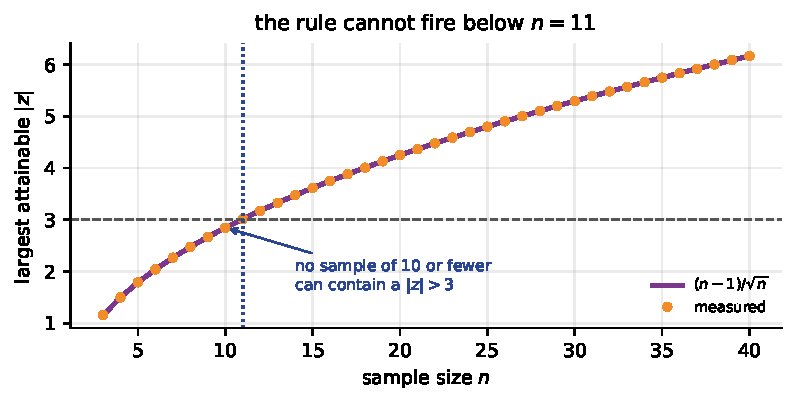
\includegraphics[width=0.56\textwidth]{maxz.pdf}
  \caption{Equation~\eqref{eq:zmax}, with the attained maxima measured
  directly. Theory and measurement agree to $9\times10^{-16}$. The crossing of
  the threshold happens between $n = 10$ and $n = 11$.}
  \label{fig:maxz}
\end{figure}

\subsection{The opposite failure: skew is not contamination}
\label{sec:skewrules}

So far the $z$-score has been too permissive. On the wrong kind of column all
three rules are far too aggressive, and for a reason that has nothing to do
with dirty data.

Take the most skewed column of \texttt{load\_breast\_cancer}: \texttt{'area
error'}, skewness $5.43$, kurtosis $48.8$, and not one contaminated value in
it.

\begin{codeout}
most skewed column of breast_cancer: 'area error', skewness 5.433
  median 24.53   mean 40.34   sd 45.49   MAD 9.19
  rule                  flags     % of rows
  |z| > 3                  6         1.1%
  1.5*IQR fences          65        11.4%
  |modified z| > 3.5      81        14.2%
  largest reading 542.2:  z = 11.03,  modified z = 38.0
  under a perfect Normal these rules flag 0.27%, 0.70% and 0.35% of rows
\end{codeout}

Eighty-one ``outliers'' out of $569$. Every one of these rules is derived under
an assumption of symmetry: the $z$-score compares a two-sided deviation with a
single $s$; the Tukey fence uses the same $1.5\,\mathrm{IQR}$ on both sides.
On a long right tail they simply flag the tail.

The fix is not a different threshold. It is to make the column symmetric first.

\begin{codeout}
  now Yeo-Johnson the column first (skewness 5.433 -> 0.069) and repeat
  |z| > 3                  0         0.0%
  1.5*IQR fences           1         0.2%
  |modified z| > 3.5       0         0.0%
\end{codeout}

\begin{figure}[tb]
  \centering
  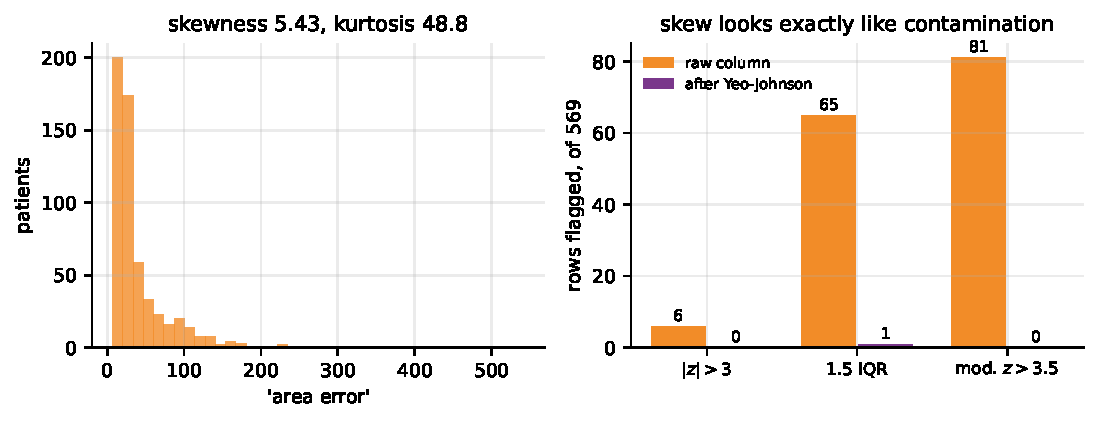
\includegraphics[width=0.84\textwidth]{rules.pdf}
  \caption{Left: the raw column. Right: how many of the 569 rows each rule
  condemns, before and after a single power transform. $6 \to 0$, $65 \to 1$,
  $81 \to 0$, and not one data value was deleted.}
  \label{fig:rules}
\end{figure}

\begin{keyidea}
Transform first, then look for outliers. An outlier rule applied to a skewed
variable is mostly a skewness detector, and if you act on it you will delete
the most informative $14\%$ of your data for being large.
\end{keyidea}

\subsection{Numerical methods for handling outliers}
\label{sec:handling}

Detection told you which points are unusual. Now: what do you do?

\subsubsection*{Binning and smoothing}

The classical treatment of \emph{noisy} numeric data --- values wrong by a
little rather than a lot --- is to sort, bin, and replace each value by a
summary of its bin.

\begin{worked}[Nine prices, three equal-depth bins]
Sorted data: $4,\ 8,\ 15,\ 21,\ 21,\ 24,\ 25,\ 28,\ 34$.

\emph{Equal-depth} (equal-frequency) binning with depth $3$ puts three values
in each bin. \emph{Equal-width} binning would instead cut the range
$[4, 34]$ into three intervals of width $10$, which here would give bins of
size $2$, $4$ and $3$.

\begin{center}
\begin{tabular}{@{}llrrl@{}}
\toprule
Bin & Values & mean & median & boundaries\\
\midrule
1 & $4,\ 8,\ 15$   & $9$  & $8$  & $4$ and $15$\\
2 & $21,\ 21,\ 24$ & $22$ & $21$ & $21$ and $24$\\
3 & $25,\ 28,\ 34$ & $29$ & $28$ & $25$ and $34$\\
\bottomrule
\end{tabular}
\end{center}

\textbf{Smoothing by bin means} replaces every value by its bin's mean:
$9, 9, 9, 22, 22, 22, 29, 29, 29$.

\textbf{Smoothing by bin medians} gives $8, 8, 8, 21, 21, 21, 28, 28, 28$ ---
and unlike the means, these are values that actually occurred.

\textbf{Smoothing by bin boundaries} replaces each value by whichever
\emph{end} of its bin is closer. In bin 1, $8$ is $4$ away from $4$ and $7$
away from $15$, so it becomes $4$; $15$ is already a boundary. The result is
$4, 4, 15, 21, 21, 24, 25, 25, 34$, which preserves the range of each bin while
flattening its interior.
\end{worked}

\begin{codeout}
sorted data  [4, 8, 15, 21, 21, 24, 25, 28, 34]
equal-frequency (equal-depth) bins of depth 3
  bin 1  [4, 8, 15]     mean  9.00   median  8   boundaries  4 and 15
  bin 2  [21, 21, 24]   mean 22.00   median 21   boundaries 21 and 24
  bin 3  [25, 28, 34]   mean 29.00   median 28   boundaries 25 and 34
smoothing by bin means       [9.0, 9.0, 9.0, 22.0, 22.0, 22.0, 29.0, 29.0, 29.0]
smoothing by bin medians     [8, 8, 8, 21, 21, 21, 28, 28, 28]
smoothing by bin boundaries  [4, 4, 15, 21, 21, 24, 25, 25, 34]
\end{codeout}

Binning is \emph{local} smoothing: it replaces a value only by something from
its own neighbourhood, so a single wild point contaminates one bin rather than
the column. That is also its limitation --- a bin of stuck readings smooths to
a stuck value.

\subsubsection*{Trim, winsorise, cap, or leave alone}

For a value that is wrong by a lot there are four choices. \textbf{Trim}:
delete the row --- loses data and, if the outliers are real, biases everything.
\textbf{Winsorise}: clip everything below the $\alpha$ percentile up to it and
everything above the $1-\alpha$ percentile down to it, keeping every row.
\textbf{Cap at a fence}: the same, but the clipping point is
$Q_3 + 1.5\,\mathrm{IQR}$, estimated from the data rather than chosen.
\textbf{Leave it and use a robust method}: a median, a
\texttt{RobustScaler}, a tree, an $L_1$ loss.

On the thirty-five sensor readings, where the truth is mean $9.586$ and
sd $0.837$:

\begin{codeout}
five ways to deal with the five stuck readings
  leave them alone         mean  22.503   sd  32.109   n 35
  winsorise at 5 and 95    mean  22.523   sd  32.100   n 35
  winsorise at 15 and 85   mean   9.903   sd   0.839   n 35
  cap at the IQR fence     mean   9.925   sd   1.143   n 35
  drop by modified z       mean   9.586   sd   0.837   n 30
  the 30 genuine readings  mean   9.586   sd   0.837   n 30
\end{codeout}

\begin{caution}[A fixed percentile is a guess about how much dirt there is]
Winsorising at the $5$th and $95$th percentiles did \textbf{nothing at all}:
mean $22.523$ against $22.503$. The contamination here is $5/35 = 14.3\%$, so
clipping the outer $5\%$ clips five stuck readings down to\dots\ other stuck
readings. Winsorising at $15$/$85$ works, and also clips five perfectly good
readings. The IQR fence and the modified $z$ need no such guess, because they
estimate the location and spread from the middle of the data and let the tails
fall where they will.
\end{caution}

\subsubsection*{Robust scaling}

The scaler you choose is an outlier decision whether you think of it that way
or not.

\begin{lstlisting}
StandardScaler().fit_transform(sensor.reshape(-1, 1))   # (x - mean) / sd
RobustScaler().fit_transform(sensor.reshape(-1, 1))     # (x - median) / IQR
\end{lstlisting}
\begin{codeout}
StandardScaler against RobustScaler on the same 35 readings
  StandardScaler  30 genuine readings span -0.4747 to -0.3527  (width 0.1220)
  RobustScaler    30 genuine readings span -2.2765 to  1.2811  (width 3.5576)
\end{codeout}

\texttt{StandardScaler} spent its entire dynamic range accommodating five wrong
numbers: the thirty good readings now occupy $0.122$ of a unit, and to any
distance-based model they are effectively identical.
\texttt{RobustScaler} centres on the median and divides by the IQR, so the
thirty good readings spread over $3.56$ units and the outliers simply sit far
away, which is where they belong.

\begin{tryit}
Run the three rules on \texttt{load\_iris} petal length: you should get zero
flags from all three. Change one value to $100$ and re-run --- all three fire,
because the single-outlier case is the one the $z$-score handles fine. Now add
a second and a third $100$ and watch the $z$-score give up.
\end{tryit}

% =========================================================================
\section{Data transformation}
\label{sec:transform}

\subsection{Why transform a variable}

Four honest reasons. \textbf{Symmetry}: a mean and a standard deviation
describe a symmetric distribution well and a skewed one badly.
\textbf{Linearity}: a relationship curved in $x$ is often straight in
$\log x$. \textbf{Constant spread}: if residual variance grows with the fitted
value, a transformation often flattens it. And \textbf{so that the outlier
rules work} --- Section~\ref{sec:skewrules}.

The bad reason is ``because everybody does''. A transformation changes what a
coefficient means, and if you cannot state the new meaning you should not
apply it.

Han, Kamber and Pei list smoothing, attribute construction, aggregation,
normalisation, discretisation and concept-hierarchy generation under the same
heading of ``data transformation''. Smoothing was Section~\ref{sec:handling};
normalisation, discretisation and attribute construction belong with feature
engineering in the next lecture. This section is about the one that changes the
\emph{shape} of a distribution.

\subsection{The ladder of powers, by hand}

Arrange the simple transformations by the power they raise $x$ to:
\[
  \dots,\quad -\frac{1}{x},\quad -\frac{1}{\sqrt x},\quad \log x,\quad
  \sqrt x,\quad x,\quad x^2,\quad x^3,\quad \dots
\]
Moving \textbf{down} the ladder pulls in a long right tail; moving \textbf{up}
pulls in a long left tail. The further you move, the stronger the effect.

\begin{worked}[Why $\log$ is the useful middle rung]
Take four values spanning two orders of magnitude: $1,\ 4,\ 16,\ 64$. They are
in geometric progression with ratio $4$, so the gaps grow: $3,\ 12,\ 48$.

Apply $\log$: $0,\ 1.3863,\ 2.7726,\ 4.1589$. The gaps are now
$1.3863,\ 1.3863,\ 1.3863$ --- exactly equal, because
$\log(4x) = \log x + \log 4$.

\textbf{The log turns multiplication into addition.} A variable whose values
are naturally \emph{ratios} --- incomes, populations, areas, concentrations,
prices --- has a skewed distribution on the original scale and a symmetric one
on the log scale, and that is not a coincidence: it is what ``multiplicative''
means. Reach for $\log$ first whenever ``twice as big'' is a more natural
statement about your variable than ``ten units bigger''.
\end{worked}

\subsection{Four transformations of one real column}

\texttt{'area error'} again: $569$ values, minimum $6.80$, maximum $542.2$,
skewness $5.43$.

\begin{lstlisting}
for name, v in (("none", col), ("sqrt", np.sqrt(col)),
                ("log", np.log(col)), ("1/sqrt", 1/np.sqrt(col))):
    print(name, stats.skew(v), stats.kurtosis(v))
\end{lstlisting}
\begin{codeout}
column 'area error',  n = 569,  min = 6.8020, max = 542.2
  transformation        skewness    kurtosis
  none                    5.4328    48.7672
  sqrt(x)                 2.1363     7.8193
  log(x)                  0.7955     0.3622
  1/sqrt(x)               0.0447    -0.3685
  Box-Cox, lam=-0.436     0.0584    -0.4094
  Yeo-Johnson             0.0691    -0.4561
\end{codeout}

Read down the skewness column: $5.43 \to 2.14 \to 0.80 \to 0.04$. The square
root was not nearly enough, the log almost did it, and the reciprocal square
root went slightly past zero.

\begin{figure}[tb]
  \centering
  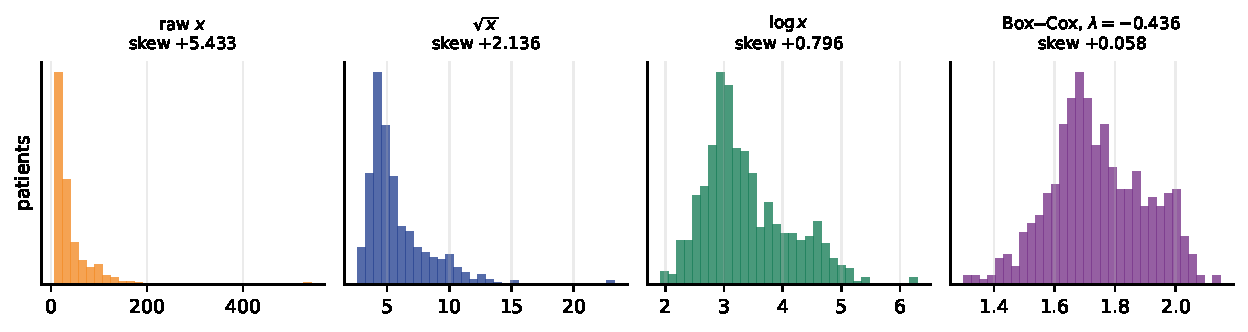
\includegraphics[width=0.94\textwidth]{transforms.pdf}
  \caption{The same 569 numbers on four different rulers. No value has been
  deleted and no value has changed its rank. Only the fourth panel is a
  variable you can sensibly summarise with a mean and a standard deviation.}
  \label{fig:transforms}
\end{figure}

The ladder is discrete, and the right rung for this column is somewhere between
$\log$ and $1/\sqrt{x}$. That gap is exactly what the next idea fills.

\subsection{Box--Cox and Yeo--Johnson}
\label{sec:boxcox}

Box and Cox (1964) embedded the whole ladder in one continuous family:
\begin{equation}
  \label{eq:boxcox}
  x^{(\lambda)} =
  \begin{cases}
    \dfrac{x^{\lambda} - 1}{\lambda}, & \lambda \neq 0,\\[8pt]
    \log x, & \lambda = 0,
  \end{cases}
  \qquad x > 0 .
\end{equation}

Two details of Equation~\eqref{eq:boxcox} are worth a moment.

\textbf{Why the $-1$ and the division by $\lambda$.} They make the family
continuous at $\lambda = 0$: without them $x^\lambda \to 1$ and the
transformation would collapse to a constant, while with them l'H\^opital's rule
gives $(x^\lambda - 1)/\lambda \to \log x$. Numerically:

\begin{codeout}
    check lambda->0:  (x**0.001 - 1)/0.001 = [0.0, 1.3873, 2.7764, 4.1675]
    log(x)                                = [0.0, 1.3863, 2.7726, 4.1589]
\end{codeout}

\textbf{Why $x > 0$.} $x^\lambda$ is not real for negative $x$ and fractional
$\lambda$ --- $(-8)^{1/2}$ does not exist in the reals --- and $\log x$ is
undefined at and below zero. A single zero or negative value in the column is
fatal, not merely awkward.

\begin{worked}[The family, on four numbers you can check in your head]
Take $x = (1, 4, 16, 64)$, a geometric sequence: each value is four times the
one before.

\begin{lstlisting}
for lam in (1.0, 0.5, 0.0, -0.5, -1.0):
    t = np.log(x) if lam == 0 else (x**lam - 1) / lam
\end{lstlisting}
\begin{codeout}
x = [ 1.  4. 16. 64.]   (deliberately a geometric sequence)
  lambda +1.00  ->  [ 0.  3. 15. 63.]
  lambda +0.50  ->  [ 0.  2.  6. 14.]
  lambda +0.00  ->  [0.     1.3863 2.7726 4.1589]
  lambda -0.50  ->  [-0.    1.    1.5   1.75]
  lambda -1.00  ->  [-0.      0.75    0.9375  0.9844]
\end{codeout}

Check one entry with a pen. At $\lambda = -0.5$ and $x = 16$:
$16^{-0.5} = 1/\sqrt{16} = 1/4 = 0.25$, so
$(0.25 - 1)/(-0.5) = (-0.75)/(-0.5) = 1.5$, which is the third entry.

Now read the $\lambda = 0$ row: $0,\ 1.3863,\ 2.7726,\ 4.1589$ --- the gaps are
all $\log 4 = 1.3863$. The log has turned a \emph{geometric} sequence into an
\emph{arithmetic} one. That is precisely what ``the log is the right ruler for
multiplicative data'' means, and it is why prices, populations and areas
usually want it.

Read down the columns instead and you can see the whole family working: as
$\lambda$ falls, the top of the range is pulled in harder and harder --- $63$,
then $14$, then $4.16$, then $1.75$. Below $\lambda = 0$ the transformation
even becomes bounded above.
\end{worked}

\subsection{Yeo--Johnson: the same idea on the whole real line}
\label{sec:yj}

Yeo and Johnson (2000) removed the positivity requirement. Their family applies
a shifted Box--Cox to the non-negative side and a mirrored copy to the negative
side, choosing the exponents so that the two halves meet smoothly at zero:

\begin{equation}
  \label{eq:yj}
  y^{(\lambda)} =
  \begin{cases}
    \dfrac{(y+1)^{\lambda} - 1}{\lambda}, & \lambda \neq 0,\ y \ge 0,\\[9pt]
    \log(y+1), & \lambda = 0,\ y \ge 0,\\[9pt]
    -\,\dfrac{(-y+1)^{2-\lambda} - 1}{2-\lambda}, & \lambda \neq 2,\ y < 0,\\[9pt]
    -\log(-y+1), & \lambda = 2,\ y < 0 .
  \end{cases}
\end{equation}

Four cases looks like a lot until you see the symmetry. The upper pair is
Box--Cox applied to $y + 1$, which is why the $\lambda = 0$ branch is
$\log(y+1)$ rather than $\log y$ --- and why it is safe at $y = 0$. The lower
pair is the same expression run backwards: negate the input, use the exponent
$2 - \lambda$ instead of $\lambda$, and negate the result. That reflection is
what makes $\lambda$ do the same job on both sides: values of $\lambda$ below
$1$ compress a right tail, and by the mirror, values above $1$ compress a left
one.

\begin{lstlisting}
probe = np.array([-3.0, -1.0, -0.5, 0.0, 0.5, 1.0, 3.0])
for lam in (0.0, 0.5, 1.0, 2.0):
    print(lam, yeo_johnson(probe, lam))
\end{lstlisting}
\begin{codeout}
x = [-3.  -1.  -0.5  0.   0.5  1.   3. ]
  lambda 0.0 -> [-7.5    -1.5    -0.625   0.      0.4055  0.6931  1.3863]
  lambda 0.5 -> [-4.6667 -1.219  -0.5581  0.      0.4495  0.8284  2.    ]
  lambda 1.0 -> [-3.  -1.  -0.5  0.   0.5  1.   3. ]
  lambda 2.0 -> [-1.3863 -0.6931 -0.4055  0.      0.625   1.5     7.5   ]

lambda = 1 is the identity on the positive side; check y(x)-x:
  [0. 0. 0. 0. 0. 0. 0.]

continuity at x = 0 for every lambda (y(0) must be 0):
  ['-0.0e+00', '0.0e+00', '0.0e+00', '0.0e+00', '0.0e+00', '0.0e+00']

our implementation vs sklearn on 'area error', lambda = -0.483636
  max |difference| = 0.000e+00
\end{codeout}

Three things in that output are worth noticing. $\lambda = 1$ leaves every
value exactly unchanged, so ``no transformation'' is a member of the family
rather than an alternative to it. Every $\lambda$ maps $0$ to $0$, so the two
halves genuinely join. And the $\lambda = 0$ and $\lambda = 2$ rows are mirror
images of one another, which is the reflection made visible.

The last line is the check that matters: Equation~\eqref{eq:yj} typed out by
hand reproduces \texttt{PowerTransformer} on all 569 values to the last bit.

\begin{caution}[Yeo--Johnson is not Box--Cox with a shift]
A common shortcut is to add a constant to make a column positive and then run
Box--Cox. That is a different transformation with a different answer, and the
shift is an extra parameter you have invented and must justify. Yeo--Johnson
needs no shift, so prefer it whenever a column can be zero or negative --- and
note that \texttt{PowerTransformer} defaults to it for exactly this reason.
\end{caution}

\subsection{How \texorpdfstring{$\lambda$}{lambda} is chosen}
\label{sec:lambda}

Both families leave one number free, and the standard answer is maximum
likelihood: assume the \emph{transformed} column is Normal, and pick the
$\lambda$ that makes it as Normal as possible. Writing $x^{(\lambda)}$ for the
transformed values and $\hat\sigma^2_\lambda$ for their variance,

\begin{equation}
  \ell(\lambda) \;=\;
  -\frac{n}{2}\log \hat\sigma^2_{\lambda}
  \;+\;
  \underbrace{(\lambda - 1)\sum_{i=1}^{n} \log x_i}_{\text{Jacobian}} .
  \label{eq:bclik}
\end{equation}

The second term is the one every summary drops, and without it the method does
not work at all. The reason is worth a sentence: the first term rewards a small
variance, and you can always make the variance smaller by choosing a $\lambda$
that squashes everything towards a point. Nothing stops it. The Jacobian term
is the change-of-variables factor from writing a density in the new units, and
it charges you for that squashing at exactly the right rate.

\begin{lstlisting}
def boxcox_loglik(x, lam):
    t = np.log(x) if lam == 0 else (x**lam - 1) / lam
    return -x.size / 2 * np.log(t.var()) + (lam - 1) * np.log(x).sum()
\end{lstlisting}
\begin{codeout}
with the Jacobian term    : lambda* = -0.4360
scipy.stats.boxcox        : lambda* = -0.4357
without the Jacobian term : lambda* = -2.0000  <-- runs to the edge

Why: dropping the Jacobian rewards any lambda that shrinks the spread,
so the 'best' transform is the one that crushes the data to a point.
The (lambda-1) * sum(log x) term is what prices that in.

variance of the transformed column at three lambdas:
   lambda -2.000   var 2.089073e-06
   lambda -0.436   var 2.458963e-02
   lambda +1.000   var 2.065795e+03
\end{codeout}

The grid search with the Jacobian lands on scipy's answer to three decimals
(the small gap is the grid spacing, not a disagreement). Delete the Jacobian
and the optimiser runs straight to the edge of the search range, because at
$\lambda = -2$ the transformed variance is $2.1\times10^{-6}$ --- four orders
of magnitude smaller than at the sensible answer, and utterly useless.

\begin{keyidea}
$\lambda$ is estimated by maximum likelihood, not chosen by you, and not chosen
to zero the skewness. It is a \textbf{learned parameter}, exactly like a mean
used for imputation --- with all the consequences for train/test discipline
that implies.
\end{keyidea}

\subsection{Two practical details that confuse everybody}

\textbf{\texttt{PowerTransformer} standardises by default.} The output has mean
$0$ and standard deviation $1$, which surprises people who expected transformed
data on something like the original scale.

\begin{codeout}
standardize=False  lambda -0.4836   mean    +1.6509   sd   0.1258   skew +0.0691
standardize=True   lambda -0.4836   mean    -0.0000   sd   1.0000   skew +0.0691

The default is True: PowerTransformer transforms AND z-scores, so the
output is centred at 0 whatever the input units were.  The skewness is
identical either way -- standardising is linear and cannot change shape.

inverse_transform round trip: max |x - back| = 1.251e-12
\end{codeout}

The skewness is identical under both settings, which it must be: standardising
is a linear rescaling and Equation~\eqref{eq:shape} is immune to those. So
\texttt{standardize=True} saves you a separate \texttt{StandardScaler} and
changes nothing about shape. And \texttt{inverse\_transform} recovers the
original values to $10^{-12}$, which is how you report a prediction back in
the units your reader cares about.

\textbf{$\lambda$ is fitted, so it belongs inside the pipeline.}

\begin{codeout}
lambda fitted on train only : -0.5527
lambda fitted on all rows   : -0.4836   (this one has seen the test set)
lambda fitted on test only  : -0.3386

The gap between the first two is small here (0.0691), but it is a
parameter learned from data, so it goes inside the Pipeline with
every other learned quantity.  Section on the order of operations.

train skew after transform +0.0981;  test skew using the TRAIN lambda -0.3051
\end{codeout}

Three splits of the same column give three different $\lambda$. Fitting on all
the rows before splitting leaks, in the same way and for the same reason as
fitting a scaler or an imputer on all the rows --- see
Section~\ref{sec:leak}. Note the last line too: applied to the test set, the
\emph{train} $\lambda$ leaves a residual skew of $-0.31$ rather than the
$+0.10$ it achieves on the data it was fitted to. That is not a bug. It is the
honest generalisation gap of a learned parameter, and hiding it by refitting on
the test set is exactly the mistake.

\begin{codeout}
diabetes 'bp': min -0.1124  max +0.1320  skew +0.2897
  stats.boxcox(bp) -> ValueError: Data must be positive.
  Yeo-Johnson handles it: skew +0.2897 -> +0.0226

a single zero is also fatal to Box-Cox: Data must be positive.
shifting by a constant is the usual workaround, and the shift is then
another parameter you have chosen and must justify.
\end{codeout}

Every named rung is a value of $\lambda$:

\begin{codeout}
Box-Cox is one family; lambda picks the member
  lambda -1.00   1/x  (reciprocal)  skewness  -0.8635
  lambda -0.50   1/sqrt(x)          skewness  -0.0447
  lambda +0.00   log(x)             skewness  +0.7955
  lambda +0.50   sqrt(x)            skewness  +2.1363
  lambda +1.00   x  (no change)     skewness  +5.4328
  maximum-likelihood lambda from scipy   -0.4357
  skewness there                         +0.0584
\end{codeout}

\begin{caution}[$\lambda$ is chosen by likelihood, not by skewness]
\texttt{scipy.stats.boxcox} picks the $\lambda$ that maximises the Gaussian
log-likelihood of the transformed data, not the one that zeroes the skewness.
On this column those are $-0.4357$ and $-0.4688$ --- close, but they are
answers to different questions, and on a heavy-tailed column they can differ a
lot. If what you need is symmetry, check the skewness afterwards rather than
assuming.
\end{caution}

\begin{figure}[tb]
  \centering
  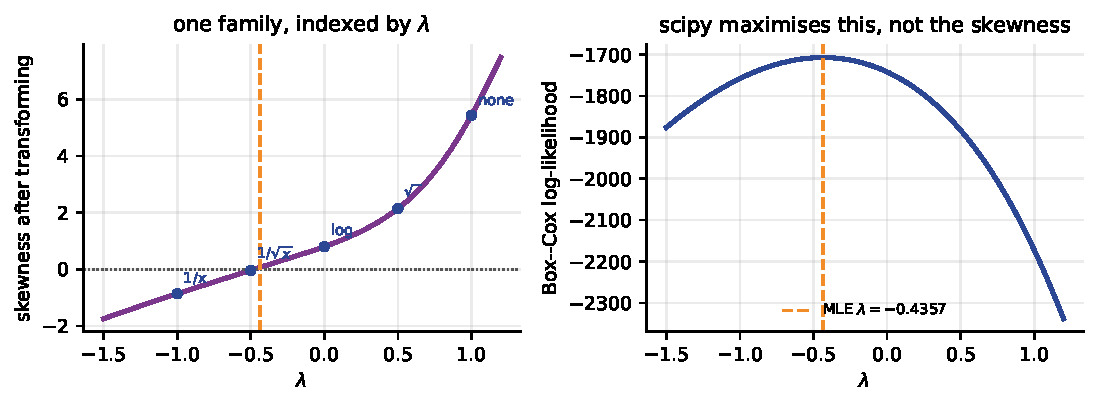
\includegraphics[width=0.84\textwidth]{boxcox.pdf}
  \caption{Left: skewness as a function of $\lambda$, with the five named rungs
  of the ladder marked. Right: the Box--Cox log-likelihood, whose maximum at
  $\lambda = -0.4357$ is what scipy returns.}
  \label{fig:boxcox}
\end{figure}

\subsection{Does it help the model?}

Sometimes, and which model it is matters more than how skewed the column was.

\begin{codeout}
does removing the skew help a model? 20 random splits
  GaussianNB           scale only 0.9304   Yeo-Johnson first 0.9462   +0.0157  (16/20)
  LogisticRegression   scale only 0.9762   Yeo-Johnson first 0.9766   +0.0003  (5/20)
\end{codeout}

Gaussian naive Bayes gains $1.6$ points on $16$ of $20$ splits, because it
\emph{assumes} each feature is Normal within each class and the transform makes
that assumption closer to true. Logistic regression gains $0.0003$ and wins $5$
splits of $20$ --- noise --- because it assumes nothing about the distribution
of the features.

\begin{keyidea}
Transform because your model assumes symmetry, because you need an outlier rule
to work, or because you need to read the variable. Not as a ritual. And when
you do transform, remember that a coefficient on $\log x$ is a statement about
percentage change, and say so in the write-up.
\end{keyidea}

\begin{tryit}
Take \texttt{load\_breast\_cancer}, compute
\texttt{stats.skew(Xb, axis=0)} and find how many of the thirty columns have
skewness above $1$. Then apply \texttt{PowerTransformer()} to the whole matrix
and count again. (You should find $12$ before and $0$ after.)
\end{tryit}

% =========================================================================
\section{The order of operations}
\label{sec:leak}

\subsection{The rule}

Everything in this lecture learns a number from the data: imputation learns a
column mean, median or mode, or a whole fitted model; outlier handling learns a
threshold, a fence, or \emph{which rows to keep}; transformation learns
$\lambda$; scaling learns a mean and a standard deviation, or a median and an
IQR.

\begin{keyidea}
Every number used to clean the data must be computed from the \textbf{training
rows only}, and then applied unchanged to the test rows. Learn it on train,
apply it everywhere: \texttt{fit} on train, \texttt{transform} on both.
\end{keyidea}

Break that and your test score stops being an estimate of performance on unseen
data, because the data was not unseen. Every course tells you that. What courses
rarely tell you is \emph{how much} it costs --- and the answer spans three
orders of magnitude depending on which step you got wrong. So we measured
three.

\subsection{Leak A: fit the scaler on everything}

The classic. \texttt{StandardScaler().fit(X)} before the split, so the mean and
standard deviation are computed from the test rows too.

\begin{lstlisting}
sc = StandardScaler().fit(Xb)                    # <-- sees the test set
m = LogisticRegression(max_iter=5000).fit(sc.transform(Xtr), ytr)
leaky = m.score(sc.transform(Xte), yte)
honest = make_pipeline(StandardScaler(),
                       LogisticRegression(max_iter=5000)
                       ).fit(Xtr, ytr).score(Xte, yte)
\end{lstlisting}
\begin{codeout}
LEAK A -- fit the scaler on everything, then split.  300 splits each
  n_train = 20  leaky 0.9338  honest 0.9304  gap +0.0034  t  +6.0  win 172/300
  n_train = 60  leaky 0.9587  honest 0.9577  gap +0.0011  t  +4.3  win 146/300
  n_train = 427 leaky 0.9774  honest 0.9772  gap +0.0002  t  +1.7  win 18/300
\end{codeout}

The leak is \textbf{real} --- at $n_{\text{train}} = 20$, $t = +6.0$ over
$300$ splits is not noise --- and \textbf{tiny}: three tenths of a percentage
point, shrinking to nothing as the training set grows, because the mean of
$427$ rows and the mean of $569$ rows are almost the same number.

\subsection{Leak B: fit the imputer on everything}

\begin{codeout}
LEAK B -- fit the imputer on everything.  30% missing, 60 splits
  mean          leaky 0.9586  honest 0.9583  gap +0.0003  t  +0.8  win 9/60
  KNN k=5       leaky 0.9535  honest 0.9552  gap -0.0017  t  -1.4  win 18/60
\end{codeout}

\begin{caution}[Report what you measured, not what you expected]
We expected KNN imputation fitted on the whole dataset to leak visibly, because
it literally copies values between rows. It did not. Over sixty splits at
$30\%$ missingness the gap was $-0.0017$ with $t = -1.4$: if anything the leaky
version scored \emph{lower}, and neither result is distinguishable from zero.

That does not make the practice acceptable. A leaky estimate is not
interpretable even when it happens not to be optimistic --- you no longer know
what it is an estimate of. But it does mean you should not go into an
examination claiming that imputing before the split produces a large
optimistic bias, because on this data it produced none.
\end{caution}

\subsection{Leak C: clean the rows using the model, then split}

Now the one that does real damage, and the one that is most human. You fit a
model, look at the rows it gets badly wrong, decide they must be outliers,
delete them, and start again.

\begin{lstlisting}
m = LinearRegression().fit(Xd, yd)             # <-- fitted on all 442 rows
res = np.abs(yd - m.predict(Xd))
keep = res <= np.quantile(res, 0.90)           # drop the worst 10%
for seed in range(0, 200):                     # a sweep: 200 different splits
    A, B, a, b = train_test_split(Xd[keep], yd[keep], test_size=0.25,
                                  random_state=seed)
    leaky = LinearRegression().fit(A, a).score(B, b)
\end{lstlisting}
\begin{codeout}
LEAK C -- drop the rows your model cannot fit, THEN split.  200 splits
  drop worst 5% leaky 0.5850  honest 0.4730  gap +0.1120  t +19.2  win 181/200
  drop worst 10% leaky 0.6390  honest 0.4688  gap +0.1702  t +29.9  win 192/200
  drop worst 20% leaky 0.7022  honest 0.4732  gap +0.2291  t +45.0  win 200/200
\end{codeout}

The honest column is the control: split first, fit on the training rows only,
drop the worst-fitted \emph{training} rows, evaluate on the untouched test set.
It barely moves --- $0.4730$, $0.4688$, $0.4732$. The leaky column climbs from
$0.4688$ to $0.7022$, and nothing about the model improved: the filter simply
removed from the \emph{test} set precisely the patients the model was going to
fail on.

\begin{keyidea}
The size of a leak is the amount of test information the step absorbs. A
column mean absorbs almost nothing --- worth $0.0034$. A decision about
\emph{which rows survive} absorbs a great deal --- worth $0.17$ of $R^2$, on
$192$ splits out of $200$. Learn to ask what the step learned from the test
set, rather than memorising a list of forbidden operations.
\end{keyidea}

\begin{figure}[tb]
  \centering
  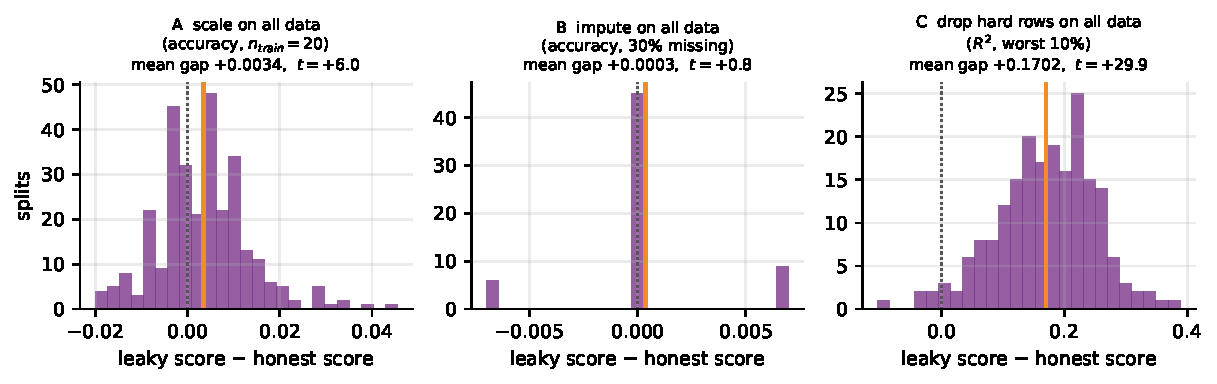
\includegraphics[width=0.94\textwidth]{leakage.pdf}
  \caption{Per-split difference, leaky minus honest, for the three sins. Note
  the horizontal scales: $0.04$, $0.008$ and $0.4$. The orange line is the
  mean, the dotted line is zero.}
  \label{fig:leakage}
\end{figure}

\subsection{The pipeline that cannot leak}

Every fix in this section is the same fix.

\begin{lstlisting}
from sklearn.pipeline import Pipeline
pipe = Pipeline([
    ("impute", SimpleImputer(strategy="median", add_indicator=True)),
    ("power",  PowerTransformer(method="yeo-johnson")),
    ("scale",  StandardScaler()),
    ("model",  LogisticRegression(max_iter=5000)),
])
print(cross_val_score(pipe, X_with_holes, y, cv=5).mean())
\end{lstlisting}
\begin{codeout}
one Pipeline, 5-fold cross-validation, 10% of cells missing
  steps: impute -> power -> scale -> model
  cross_val_score  0.9578  +/- 0.0140
every step is refitted inside every fold, so no fold ever sees its own
test rows -- and there is nothing left for you to get wrong by hand
\end{codeout}

\texttt{cross\_val\_score} calls \texttt{fit} on the pipeline five times, once
per fold. Each time the medians, the $\lambda$s, the means and the standard
deviations are recomputed from four fifths of the data, and the held-out fifth
is only ever passed to \texttt{transform}. You cannot get the order wrong,
because you no longer write the order.

\begin{caution}[Row-dropping does not fit in a Pipeline, and that is the point]
A scikit-learn transformer may change the columns of $X$ but not its rows, so
there is no \texttt{OutlierRemover} step you can slot in. That is a design
decision, not an omission: dropping rows during \texttt{transform} would break
the correspondence with $y$, and dropping them from the test fold is exactly
Leak C. If you must remove outliers, do it to the training set, by hand, after
the split --- and evaluate on everything.
\end{caution}

\begin{tryit}
Reproduce Leak C for yourself with ten random seeds. Then change the honest
version so that it also drops the worst-fitted rows from the \emph{test} set,
and watch it become the leaky version. Being able to write the bug deliberately
is the best evidence that you will not write it accidentally.
\end{tryit}

% =========================================================================
\section{Summary}

\begin{enumerate}[leftmargin=*]
  \item Listwise deletion survives with probability $(1-p)^d$, exponential in
    the number of columns. Five per cent of cells missing across thirty
    features left $114$ patients of $569$.
  \item Mean imputation leaves the mean alone and multiplies the variance by
    exactly $m/n$: measured $0.9486$ against $\sqrt{0.9} = 0.9487$ and $0.5447$
    against $\sqrt{0.3} = 0.5477$. The shrinkage propagates ---
    $\mathrm{corr}(\mathrm{BMI}, y)$ fell from $0.5865$ to $0.4538$ at $40\%$
    imputed.
  \item MCAR / MAR / MNAR is the only taxonomy that changes what you can do.
    Complete-case bias was $-0.10$, $+1.35$ and $-2.95\ \mathrm{kg/m^2}$;
    MICE fixed the MAR case ($+1.35 \to -0.16$) and could not fix MNAR
    ($-2.95 \to -2.58$).
  \item Under MNAR, mean imputation flipped the sign of a regression
    coefficient: $+5.603$ became $-0.413$.
  \item Dropping incomplete rows cost $0.05$ of $R^2$ at $10\%$ missingness
    and $5.17$ at $30\%$. The choice among five imputers cost $0.003$.
    \textbf{Spend your attention accordingly.}
  \item \texttt{add\_indicator=True} was worth $+0.1675$ of accuracy when the
    missingness itself carried the signal.
  \item \textbf{Thirty good sensor readings plus five stuck at $100$: the
    $|z|>3$ rule flagged none of them} ($z = 2.4135$). The IQR fence flagged
    five plus one false positive; the modified $z$ flagged exactly five, at
    $M = 112.5$.
  \item Masking is monotone: one outlier is caught at $z = 5.38$, three barely
    at $3.11$, and from four onwards the rule never fires again. And no sample
    can contain a $|z|$ larger than $(n-1)/\sqrt n$, so for $n \le 10$ the rule
    $|z| > 3$ is not strict but inert.
  \item On a column with skewness $5.43$ and no contamination, the three rules
    flagged $6$, $65$ and $81$ rows of $569$. After one Yeo--Johnson: $0$, $1$
    and $0$. \textbf{Transform first, then look for outliers.}
  \item Box--Cox found $\lambda = -0.4357$ by maximum likelihood and took the
    skewness from $5.4328$ to $0.0584$. Every named rung of the ladder is a
    value of $\lambda$; Yeo--Johnson is the version that survives negative
    values.
  \item Removing the skew was worth $+0.0157$ to Gaussian naive Bayes, which
    assumes normality, and $+0.0003$ to logistic regression, which does not.
  \item Leaking the scaler was worth $+0.0034$ ($t = 6.0$); leaking the imputer
    was worth nothing measurable; leaking a row-dropping decision was worth
    $+0.1702$ of $R^2$ ($t = 29.9$). Use a \texttt{Pipeline} and none of them
    can happen.
\end{enumerate}

% =========================================================================
\section{Practice questions}

Attempt these before reading Section~\ref{sec:solutions}. Questions 1, 4, 5, 6
and 7 are pure hand arithmetic and are the ones most likely to appear on a
paper.

\begin{enumerate}[leftmargin=*]
  \item\label{q:impute} Five lab scores out of $25$ are recorded as
    $18,\ 22,\ ?,\ 15,\ ?$. (a) Compute the mean, the median and the sample
    standard deviation of what was observed. (b) Impute both holes with the
    mean, then with the median, and recompute the mean and standard deviation
    in each case. (c) Check your standard deviation against the formula of
    Section~\ref{sec:shrink}.

  \item\label{q:mech} A household survey asks for annual income. Thirty per
    cent of respondents leave it blank, and follow-up shows the blanks are
    concentrated among the highest earners. (a) Name the mechanism. (b) What
    does complete-case analysis do to the estimated mean income --- which
    direction, and can you bound it? (c) The survey also records occupation and
    postcode, both complete. Under what circumstance would
    \texttt{IterativeImputer} fix the problem, and why does it not fix it here?

  \item\label{q:listwise} A table has $d$ columns and each cell is
    independently missing with probability $p$. (a) Write down the probability
    a row survives listwise deletion. (b) At $p = 0.05$, how many columns
    before you expect to lose half the rows? (c) You have $50$ columns and
    $p = 0.10$; you need $1000$ complete rows. How many rows must you collect?

  \item\label{q:rules} Twelve measurements, already sorted:
    \[ 41,\ 44,\ 45,\ 47,\ 48,\ 49,\ 51,\ 52,\ 54,\ 57,\ 120,\ 125. \]
    Compute the mean, sample standard deviation, median, MAD, $Q_1$, $Q_3$ and
    the Tukey fences. Then score $120$ and $125$ with all three rules of
    Section~\ref{sec:rules} and say which rule flags what. Explain the result.

  \item\label{q:ceiling} Prove that $|z_i| \le (n-1)/\sqrt{n}$ for any sample
    of size $n$ using the $n-1$ standard deviation. What is the smallest $n$
    for which a rule of $|z| > 3$ can ever fire? What about $|z| > 2$?

  \item\label{q:bin} Smooth the twelve values
    $8,\ 9,\ 15,\ 16,\ 16,\ 20,\ 21,\ 21,\ 24,\ 26,\ 27,\ 30$ using
    equal-depth bins of depth $3$, by bin means, by bin medians and by bin
    boundaries. Which of the three never invents a value that did not occur in
    the data?

  \item\label{q:bc} Apply the Box--Cox transformation of
    Equation~\eqref{eq:boxcox} to $x = 1,\ 4,\ 16,\ 64$ for
    $\lambda = 1,\ 0.5,\ 0,\ -1$. (a) Why is the first transformed value zero
    in every case? (b) Show numerically that the $\lambda \neq 0$ formula tends
    to $\log x$ as $\lambda \to 0$. (c) Why does the same formula fail on the
    diabetes \texttt{bp} column, and what do you use instead?

  \item\label{q:wins} On the thirty-five sensor readings of
    Section~\ref{sec:masking}, winsorising at the $5$th and $95$th percentiles
    changed the mean from $22.503$ to $22.523$ --- effectively nothing.
    Explain why, and state the general rule for choosing a winsorising
    percentile. What would you use instead if you did not know the
    contamination rate?

  \item\label{q:debug} A colleague reports $R^2 = 0.64$ on the diabetes data
    with an ordinary linear regression. You reproduce their code and get
    $0.47$. Their notebook, in order, does: (i) load the data; (ii) fit a
    linear model to all $442$ rows and delete the $10\%$ with the largest
    residual; (iii) \texttt{StandardScaler().fit\_transform(X)} on what is
    left; (iv) \texttt{train\_test\_split}; (v) fit and report. Identify every
    problem, say which one accounts for essentially all of the gap, and give
    the corrected code.

  \item\label{q:design} You are handed a table of $8000$ patient records with
    $40$ numeric columns. Twelve per cent of the cells are missing; three
    columns have skewness above $4$; one column is a laboratory value that is
    recorded only when a clinician orders the test. Design the cleaning
    pipeline. For each decision, cite a measured number from this lecture that
    supports it.
\end{enumerate}

% =========================================================================
\section{Solutions}
\label{sec:solutions}

\textbf{1.} Observed: $18,\ 22,\ 15$, so $m = 3$ and $n = 5$.

(a) Mean $= 55/3 = 18.3333$ and median $= 18$. For the sample standard
deviation, the deviations are $-0.3333$, $3.6667$ and $-3.3333$; their squares
sum to $0.1111 + 13.4444 + 11.1111 = 24.6667$; dividing by $m - 1 = 2$ gives
$12.3333$, so $s = 3.5119$.

(b) Mean-imputed: $18,\ 22,\ 18.3333,\ 15,\ 18.3333$. The mean is unchanged at
$18.3333$; the standard deviation is $2.4833$. Median-imputed:
$18,\ 22,\ 18,\ 15,\ 18$, whose mean has \emph{moved} to $18.2$ and whose
standard deviation is $2.4900$.

(c) $\sqrt{(m-1)/(n-1)} = \sqrt{2/4} = 0.7071$, and
$2.4833/3.5119 = 0.7071$. Exact.

\begin{codeout}
Q1  observed [18.0, 22.0, 15.0]  m=3  n=5
    mean 18.3333   median 18.0000   sd(ddof=1) 3.5119
    mean   imputed: mean 18.3333  sd 2.4833  ratio 0.7071
    median imputed: mean 18.2000  sd 2.4900  ratio 0.7090
    sqrt((m-1)/(n-1)) = sqrt(2/4) = 0.7071
\end{codeout}

Note that the median-imputed ratio, $0.7090$, is \emph{not} exactly
$\sqrt{0.5}$. The derivation in Section~\ref{sec:shrink} used the fact that the
filled value contributes zero deviation, which is only true for the mean.

\medskip
\textbf{2.} (a) \textbf{MNAR}: the probability of a value being missing depends
on the value itself.

(b) It \textbf{underestimates} mean income, because the discarded
observations are systematically the large ones. You cannot bound the bias from
the data --- that is what MNAR means --- but you can bound it from outside: a
known population maximum or a tax authority's aggregate gives a worst case. A
sensitivity analysis over plausible assumptions is the standard practice.

(c) \texttt{IterativeImputer} learns $P(\text{income} \mid \text{occupation},
\text{postcode})$ \emph{from the respondents who answered}. If, within any
given occupation and postcode, the answerers and the refusers had the same
income distribution, the mechanism would be MAR and the imputer would recover
the truth. Here a high earner refuses \emph{because} they are a high earner, so
within every occupation and postcode the observed incomes are the low ones and
the imputer faithfully reproduces the bias. Measured: MAR bias
$+1.3473 \to -0.1588$ under MICE, MNAR bias $-2.9505 \to -2.5834$.

\medskip
\textbf{3.} (a) $P = (1-p)^d$.

(b) $(0.95)^d = 0.5$ gives $d = \log 0.5 / \log 0.95 = 13.5$, so from about
fourteen columns onwards you are discarding more than half your data.

(c) $(0.90)^{50} = 0.00515$, so you need $1000/0.00515 = 194{,}000$ rows to end
up with $1000$ complete ones. If that sounds absurd, it is --- and it is the
argument for imputation in one line.

\begin{codeout}
Q3  rows surviving listwise deletion, (1-p)**d
    d= 5   p=0.01 0.951   p=0.05 0.774   p=0.10 0.590   half-life d at p=0.05: 13.5
    d=10   p=0.01 0.904   p=0.05 0.599   p=0.10 0.349   half-life d at p=0.05: 13.5
    d=20   p=0.01 0.818   p=0.05 0.358   p=0.10 0.122   half-life d at p=0.05: 13.5
    d=30   p=0.01 0.740   p=0.05 0.215   p=0.10 0.042   half-life d at p=0.05: 13.5
    d=50   p=0.01 0.605   p=0.05 0.077   p=0.10 0.005   half-life d at p=0.05: 13.5
\end{codeout}

\medskip
\textbf{4.} The mean is $733/12 = 61.0833$ and the sample standard deviation is
$29.0406$ --- both dragged upwards by the last two values. The median is
$(49+51)/2 = 50$. Absolute deviations from $50$ are
$9, 6, 5, 3, 2, 1, 1, 2, 4, 7, 70, 75$; their median is $4.5$, so
$\mathrm{MAD} = 4.50$. The quartiles are $Q_1 = 46.50$ and $Q_3 = 54.75$, so
$\mathrm{IQR} = 8.25$ and the fences are $34.125$ and $67.125$.

\begin{codeout}
Q4  n=12  mean 61.0833  sd 29.0406  median 50.00  MAD 4.50
    Q1 46.50  Q3 54.75  IQR 8.25  fences 34.125 and 67.125
    z of 120 = 2.0288   z of 125 = 2.2009   ceiling (n-1)/sqrt(n) = 3.1754
    modified z of 120 = 10.49   of 125 = 11.24
    flags:  |z|>3 0      IQR 2      |mod z|>3.5 2
    with the two large values removed: sd 4.8488, z of 120 would be 14.7
\end{codeout}

The $z$-scores are $2.03$ and $2.20$, both comfortably inside the threshold, so
$|z| > 3$ flags \textbf{nothing}. Both other rules flag both points. Two
explanations, and you should give both.

\emph{Masking.} The two large values inflated $s$ from $4.85$ (on the ten
genuine measurements) to $29.04$, a factor of six; divided by the
uncontaminated $s$, $120$ would score $z = 14.7$. \emph{The ceiling.} With
$n = 12$ the largest attainable $|z|$ is $11/\sqrt{12} = 3.1754$, so even a
value of $10^{9}$ would have scored only $3.18$ --- the rule had almost no room
to work in even before the masking.

\medskip
\textbf{5.} Write $d_i = x_i - \bar x$, so $\sum_i d_i = 0$ and
$\sum_i d_i^2 = (n-1)s^2$. Fix attention on $d_1$. The other $n-1$ deviations
sum to $-d_1$, and for a fixed sum the sum of squares is minimised when they
are all equal, so $\sum_{i\ge2} d_i^2 \ge d_1^2/(n-1)$. Hence
\[
  (n-1)s^2 \;\ge\; d_1^2 + \frac{d_1^2}{n-1} = d_1^2 \cdot \frac{n}{n-1},
  \qquad\text{so}\qquad
  \frac{d_1^2}{s^2} \le \frac{(n-1)^2}{n},
  \qquad |z_1| \le \frac{n-1}{\sqrt n}.
\]
For $|z| > 3$ we need $(n-1)/\sqrt n > 3$, i.e.\ $n - 1 > 3\sqrt n$. At
$n = 10$, $9/\sqrt{10} = 2.846$; at $n = 11$, $10/\sqrt{11} = 3.015$. So
\textbf{$n \ge 11$}. For $|z| > 2$: at $n = 5$, $4/\sqrt5 = 1.789$; at $n = 6$,
$5/\sqrt6 = 2.041$. So $n \ge 6$.

\medskip
\textbf{6.} Depth $3$ gives four bins.

\begin{codeout}
Q6  sorted [8, 9, 15, 16, 16, 20, 21, 21, 24, 26, 27, 30]
    bin 1 [8, 9, 15]     mean  10.67  median  9  boundaries  8,15
    bin 2 [16, 16, 20]   mean  17.33  median 16  boundaries 16,20
    bin 3 [21, 21, 24]   mean  22.00  median 21  boundaries 21,24
    bin 4 [26, 27, 30]   mean  27.67  median 27  boundaries 26,30
    by means      [10.67, 10.67, 10.67, 17.33, 17.33, 17.33, 22.0, 22.0, 22.0, 27.67, 27.67, 27.67]
    by medians    [9, 9, 9, 16, 16, 16, 21, 21, 21, 27, 27, 27]
    by boundaries [8, 8, 15, 16, 16, 20, 21, 21, 24, 26, 26, 30]
\end{codeout}

Check bin 1 by hand: $8, 9, 15$ has mean $32/3 = 10.67$ and median $9$; for the
boundaries, $9$ is $1$ from $8$ and $6$ from $15$, so it becomes $8$.
\textbf{Bin medians and bin boundaries never invent a value}; bin means can
produce $10.67$ when every measurement was an integer, which matters if the
column is a count or a category code.

\medskip
\textbf{7.} (a) $x = 1$ gives $(1^\lambda - 1)/\lambda = 0$ for every
$\lambda \neq 0$, and $\log 1 = 0$. The $-1$ in the numerator is what fixes the
value $1$ to map to $0$ throughout the family.

\begin{codeout}
Q7  x = [1.0, 4.0, 16.0, 64.0]
    lambda +1.0 -> [0.0, 3.0, 15.0, 63.0]
    lambda +0.5 -> [0.0, 2.0, 6.0, 14.0]
    lambda +0.0 -> [0.0, 1.3863, 2.7726, 4.1589]
    lambda -1.0 -> [0.0, 0.75, 0.9375, 0.9844]
\end{codeout}

Check $\lambda = 0.5$ by hand: $(\sqrt{4} - 1)/0.5 = (2-1)/0.5 = 2$;
$(\sqrt{16}-1)/0.5 = 6$; $(\sqrt{64}-1)/0.5 = (8-1)/0.5 = 14$. Notice how the
spacing changes: at $\lambda = 1$ the gaps are $3, 12, 48$; at $\lambda = 0$
they are equal. That is the ladder working.

(b) Put $\lambda = 0.001$:

\begin{codeout}
    check lambda->0:  (x**0.001 - 1)/0.001 = [0.0, 1.3873, 2.7764, 4.1675]
    log(x)                                = [0.0, 1.3863, 2.7726, 4.1589]
\end{codeout}

Agreement to three decimals, improving as $\lambda \to 0$: analytically
$x^\lambda = e^{\lambda \log x} = 1 + \lambda\log x + O(\lambda^2)$.

(c) The diabetes \texttt{bp} column runs from $-0.1124$ to $+0.1320$ and
$x^{\lambda}$ is not real for negative $x$ at fractional $\lambda$; scipy
raises \texttt{ValueError: Data must be positive}. Use Yeo--Johnson, which took
the skewness from $+0.2897$ to $+0.0226$. Shifting the column by a constant and
then using Box--Cox is a common alternative, but the answer then depends on the
shift, which is one more thing to justify.

\medskip
\textbf{8.} Winsorising at $\alpha = 5\%$ clips the outer $5\%$ of the
\emph{sample}, but the contamination here is $5/35 = 14.3\%$. Clipping the top
$5\%$ means clipping the top $1.75$ observations --- all of them stuck readings
at $100$ --- down to the $95$th percentile, which is \emph{also} a stuck
reading at $100$. Nothing moves.

\begin{codeout}
Q8  winsorising the 35 sensor readings at symmetric percentiles
     2/98  mean  22.515  sd  32.104   (truth 9.586 / 0.837)
     5/95  mean  22.523  sd  32.100   (truth 9.586 / 0.837)
    10/90  mean  22.569  sd  32.079   (truth 9.586 / 0.837)
    15/85  mean   9.903  sd   0.839   (truth 9.586 / 0.837)
    20/80  mean   9.824  sd   0.565   (truth 9.586 / 0.837)
    contamination is 5/35 = 14.3%
\end{codeout}

The general rule: \textbf{$\alpha$ must exceed the contamination rate}, which
you rarely know, so you are guessing. Overshoot and you clip good data --- at
$20$/$80$ the standard deviation falls to $0.565$ against a true $0.837$,
because sixteen genuine readings have been clipped. If you do not know the
rate, use a rule that estimates the centre and spread from the middle of the
data rather than from a fixed tail quantile: the $1.5\,\mathrm{IQR}$ fence gave
mean $9.925$, and the modified $z$-score recovered the thirty genuine readings
exactly.

\medskip
\textbf{9.} There are three problems, and they are not equally serious.

\emph{Problem 1, and it is the whole gap.} Step (ii) fits a model to all $442$
rows and deletes the ones it fits worst, \emph{before} the split. Those rows are
then absent from the test set, so the test set no longer contains the patients
the model would fail on. Measured over $200$ splits, this alone moves $R^2$
from $0.4688$ to $0.6390$: a gap of $+0.1702$ with $t = 29.9$, and the leaky
number wins on $192$ of the $200$. It accounts for essentially all of the
$0.64$ against $0.47$.

\emph{Problem 2, real but small.} Step (iii) fits the scaler on all surviving
rows, so the test rows contribute to the mean and standard deviation. Measured
separately: $+0.0034$ at a training set of $20$ rows, $+0.0002$ at $427$ ---
detectable, practically irrelevant here, and free to fix.

\emph{Problem 3, not leakage but still wrong.} Deleting the worst-fitted
$10\%$ defines ``outlier'' as ``inconvenient for my model'', which guarantees
the survivors agree with the model. Even done correctly, inside the training
set only, it buys nothing: $0.4730$, $0.4688$, $0.4732$ for $5\%$, $10\%$ and
$20\%$.

Corrected:

\begin{lstlisting}
X_tr, X_te, y_tr, y_te = train_test_split(X, y, test_size=0.25,
                                          random_state=0)
model = make_pipeline(StandardScaler(), LinearRegression())
model.fit(X_tr, y_tr)                     # scaler fitted on train only
print(model.score(X_te, y_te))            # evaluated on every test row
\end{lstlisting}

If outlier removal is genuinely wanted, do it to \texttt{X\_tr} and
\texttt{y\_tr} after the split, with a criterion that does not consult the
model --- the modified $z$-score, say --- and never touch \texttt{X\_te}.

\medskip
\textbf{10.} A defensible pipeline, with the evidence for each step.

\emph{Look before you clean.} Count missing cells per column and per row and
plot every histogram. At $12\%$ per cell across $40$ columns, listwise deletion
keeps $(0.88)^{40} = 0.6\%$ of the rows --- $48$ patients of $8000$. That one
line of arithmetic settles whether to delete.

\emph{Missing values.} Impute, with the median, because three columns are
strongly skewed. Which imputer barely matters: our measured spread across five
was $0.003$ of $R^2$ at $10\%$ missingness against $0.05$ for deletion.
Consider \texttt{KNNImputer} if $12\%$ behaves like our $30\%$ case, where KNN
gave $0.4591$ against mean imputation's $0.4351$ --- but watch the variance,
since MICE there gave $0.2639 \pm 0.5004$.

\emph{The clinician-ordered laboratory value.} Set
\texttt{add\_indicator=True}: when missingness carried signal it was worth
$+0.1675$ of accuracy (Section~\ref{sec:indicator}). Then ask whether the test
is ordered \emph{because} of something already known about the outcome --- if
so the indicator is leakage and must go. Suspect MNAR here and say so: our MNAR
case flipped a coefficient from $+5.603$ to $-0.413$.

\emph{Skew, before outliers.} Apply \texttt{PowerTransformer} (Yeo--Johnson, so
negative values are safe) to the three skewed columns. On a column with
skewness $5.43$ this cut the rows flagged as outliers from $6$, $65$ and $81$
to $0$, $1$ and $0$; running an outlier rule first would have deleted the top
$14\%$ of a legitimate distribution.

\emph{Outliers.} Use the modified $z$-score, not $|z| > 3$: on our sensor data
the $z$ rule found zero of five obvious outliers and the modified $z$ found
exactly five. Investigate rather than delete. If a flagged value is impossible,
drop that row from the training set only; if it is merely large, keep it and
use \texttt{RobustScaler}, which kept the thirty genuine readings spread over
$3.56$ units where \texttt{StandardScaler} squeezed them into $0.122$.

\emph{Order.} Everything except the row deletion goes into one
\texttt{Pipeline}; the row deletion happens by hand after the split, on the
training set only. Measured cost of getting this wrong: $+0.0034$ for a leaked
scaler, $+0.1702$ for a leaked row-dropping decision.

% =========================================================================
\section{References and further reading}

All links were checked on 22 August 2026. Free resources are marked
\textbf{[free]}.

\subsection*{Textbooks}

\begin{itemize}[leftmargin=*]
  \item Han, Kamber and Pei, \emph{Data Mining: Concepts and Techniques}, 3rd
    edition, Morgan Kaufmann, 2012. \textbf{The prescribed text.} \S3.1 the
    four preprocessing tasks; \S3.2 data cleaning, with \S3.2.1 missing values
    and \S3.2.2 the binning and smoothing of Section~\ref{sec:handling};
    \S3.5 data transformation and discretisation.
  \item M\"uller and Guido, \emph{Introduction to Machine Learning with
    Python}, O'Reilly, 2016. Ch.~4 on representing data; \S6.1--6.2 make the
    \texttt{Pipeline} argument of Section~\ref{sec:leak}. Notebooks
    \textbf{[free]}:
    \url{https://github.com/amueller/introduction_to_ml_with_python}
  \item Wes McKinney, \emph{Python for Data Analysis}, 3e. \textbf{[free]}
    Ch.~7 ``Data Cleaning and Preparation'' --- the pandas half of this
    lecture: missing data, replacing, \texttt{pd.cut}/\texttt{pd.qcut},
    detecting outliers. \url{https://wesmckinney.com/book/data-cleaning}
  \item Stef van Buuren, \emph{Flexible Imputation of Missing Data}, 2e.
    \textbf{[free]} The standard reference, by the author of \texttt{mice}.
    \S1.2 MCAR/MAR/MNAR; \S1.3.1--1.3.3 listwise deletion and mean imputation,
    with the variance argument of Section~\ref{sec:shrink}; \S1.3.7 the
    indicator method; \S4.5.2 the MICE algorithm.
    \url{https://stefvanbuuren.name/fimd/}
  \item Kuhn and Johnson, \emph{Feature Engineering and Selection}.
    \textbf{[free]} Ch.~6 Box--Cox and Yeo--Johnson in practice; Ch.~8 missing
    data. \url{http://www.feat.engineering/}
  \item James et al., \emph{An Introduction to Statistical Learning with
    Python}. \textbf{[free]} \S3.3.3 outliers and high-leverage points in
    regression --- why Leak C is so seductive.
    \url{https://www.statlearning.com/}
\end{itemize}

\subsection*{Online courses}

\begin{sloppypar}
\begin{itemize}[leftmargin=*]
  \item \textbf{NPTEL, Data Mining} --- Prof.\ Pabitra Mitra, IIT Kharagpur.
    Lectures 2 and 3 are ``Data Preprocessing I'' and ``II'', the closest
    match to this lecture on NPTEL. \textbf{[free]}
    \url{https://nptel.ac.in/courses/106105174}
  \item \textbf{NPTEL, Introduction to Machine Learning} --- Prof.\ Balaraman
    Ravindran, IIT Madras; the reference course for the semester.
    \textbf{[free]} \url{https://nptel.ac.in/courses/106106139}
  \item \textbf{SWAYAM} --- the national portal hosting NPTEL. \textbf{[free]}
    \url{https://swayam.gov.in/}
  \item \textbf{Kaggle Learn, Data Cleaning} --- four hands-on browser lessons
    (missing values, scaling, dates, inconsistent entry), two or three hours,
    and a good complement to the Google crash course. \textbf{[free]}
    \url{https://www.kaggle.com/learn/data-cleaning} \\
    \url{https://developers.google.com/machine-learning/crash-course}
\end{itemize}
\end{sloppypar}

\subsection*{Videos}

\begin{itemize}[leftmargin=*]
  \item Data Mining --- IITKGP (NPTEL, Prof.\ Pabitra Mitra), \emph{Lecture 3
    Data Preprocessing - II}: data quality and the preprocessing steps at the
    board, in the vocabulary you will be examined in. \textbf{[free]}
    \url{https://youtu.be/wZQM_9vhulg}, after \emph{Lecture 2 Data
    Preprocessing - I} \url{https://youtu.be/NSxEiohAH5o}
  \item Stats with Mia, \emph{Missing Data Assumptions (MCAR, MAR, MNAR)} ---
    the clearest short account of Section~\ref{sec:mechanisms}.
    \textbf{[free]} \url{https://youtu.be/YpqUbirqFxQ}
  \item AnalytiCode, \emph{Modified Z-Score Explained (Python Outlier
    Detection)} --- exactly the failure of Section~\ref{sec:masking}, and the
    fix. \textbf{[free]} \url{https://youtu.be/wCXQo6OYbhg}
  \item Phil Chan, \emph{Transforming the response(Y) in regression: Box Cox
    transformation (7 mins)}. \textbf{[free]}
    \url{https://youtu.be/zYeTyEWt7Cw}
\end{itemize}

\subsection*{Documentation and interactive explainers}

\begin{itemize}[leftmargin=*]
  \item scikit-learn user guide: \emph{Imputation of missing values}
    (\texttt{SimpleImputer}, \texttt{IterativeImputer}, \texttt{KNNImputer},
    \texttt{MissingIndicator}); \emph{Preprocessing data}
    (\texttt{PowerTransformer}, \texttt{RobustScaler}); \emph{Pipelines and
    composite estimators}. \textbf{[free]}
    \url{https://scikit-learn.org/stable/modules/impute.html} \\
    \url{https://scikit-learn.org/stable/modules/preprocessing.html} \\
    \url{https://scikit-learn.org/stable/modules/compose.html}
  \item scikit-learn, \emph{Common pitfalls and recommended practices} --- read
    the section on inconsistent preprocessing before you next report a score.
    \textbf{[free]} \url{https://scikit-learn.org/stable/common_pitfalls.html}
  \item Three scikit-learn examples: \emph{Compare the effect of different
    scalers on data with outliers}; \emph{Map data to a normal distribution};
    \emph{Imputing missing values before building an estimator}.
    \textbf{[free]}
    \url{https://scikit-learn.org/stable/auto_examples/preprocessing/plot_all_scaling.html}
    \\
    \url{https://scikit-learn.org/stable/auto_examples/preprocessing/plot_map_data_to_normal.html}
    \\
    \url{https://scikit-learn.org/stable/auto_examples/impute/plot_missing_values.html}
  \item pandas user guide, \emph{Working with missing data}; and
    \texttt{scipy.stats.boxcox} for the maximum-likelihood $\lambda$ (with
    \texttt{boxcox\_llf} for Figure~\ref{fig:boxcox}). \textbf{[free]}
    \url{https://pandas.pydata.org/docs/user_guide/missing_data.html} \\
    \url{https://docs.scipy.org/doc/scipy/reference/generated/scipy.stats.boxcox.html}
\end{itemize}

\subsection*{Articles}

\begin{itemize}[leftmargin=*]
  \item NIST/SEMATECH, \emph{e-Handbook of Statistical Methods}, \S1.3.5.17
    ``Detection of Outliers'' --- the authoritative free source for
    Section~\ref{sec:outliers}: the $(n-1)/\sqrt{n}$ ceiling, masking and
    swamping, and the modified $z$-score. \textbf{[free]}
    \url{https://www.itl.nist.gov/div898/handbook/eda/section3/eda35h.htm}
  \item Brownlee, ``Data Leakage in Machine Learning'' --- a checklist for
    Section~\ref{sec:leak}. \textbf{[free]}
    \url{https://machinelearningmastery.com/data-leakage-machine-learning/}
\end{itemize}

\enlargethispage{4\baselineskip}
\notesources{\AMLUnitIVSources}

\end{document}
